% options:
% thesis=B bachelor's thesis
% thesis=M master's thesis
% czech thesis in Czech language
% slovak thesis in Slovak language
% english thesis in English language
% hidelinks remove colour boxes around hyperlinks

\documentclass[thesis=B,czech]{FITthesis}[2012/06/26]

\usepackage[utf8]{inputenc} % LaTeX source encoded as UTF-8

\usepackage{graphicx} % graphics files inclusion
\usepackage{amsmath} % advanced maths
\usepackage{amssymb} % additional math symbols

\hypersetup{unicode}

\usepackage{dirtree} % directory tree visualisation

% % list of acronyms
\usepackage[acronym,nonumberlist,toc,numberedsection=autolabel]{glossaries}
\iflanguage{czech}{\renewcommand*{\acronymname}{Seznam pou{\v z}it{\' y}ch zkratek}}{}
\makeglossaries

\newcommand{\tg}{\mathop{\mathrm{tg}}} %cesky tangens
\newcommand{\cotg}{\mathop{\mathrm{cotg}}} %cesky cotangens

% % % % % % % % % % % % % % % % % % % % % % % % % % % % % % 
% ODTUD DAL VSE ZMENTE
% % % % % % % % % % % % % % % % % % % % % % % % % % % % % % 

%%%%%%%%%%%%%%%%%%%%%%%%%%%%%%%%%%%%%%%%%%%%%%%%%%%%%%%%%%%% <nesrotom>

\providecommand{\e}[1]{\ensuremath{\times 10^{#1}}}

%the worse package ever made.
%\usepackage{float}

\usepackage{algorithm}% http://ctan.org/pkg/algorithms
\usepackage{algpseudocode}% http://ctan.org/pkg/algorithmicx
\usepackage{pseudocode}

\let\mylistof\listof
\renewcommand\listof[2]{%
\mylistof{algorithm}{Seznam algoritmů}%
}

% macro to define a local label
%\newcommand\locallabel[1]{\label{\currentprefix:#1}}
% macro to use a local reference
%\newcommand\localref[1]{\ref{\currentprefix:#1}}

%\mylistof{algorithm}{}

\newcommand{\bigO}{\ensuremath{\mathcal{O}}}

\usepackage{rotating}


%%%%%%%%%%%%%%%%%%%%%%%%%%%%%%%%%%%%%%%%%%%%%%%%%%%%%%%%%%%% </nesrotom>

\department{Katedra Teoretické informatiky}
\title{Vliv formátu uložení řídké matice na výkonnost násobení řídkých matic}
\authorGN{Tomáš} %(křestní) jméno (jména) autora
\authorFN{Nesrovnal} %příjmení autora
\authorWithDegrees{Tomáš Nesrovnal} %jméno autora včetně současných akademických titulů
\supervisor{Ing. Ivan Šimeček, Ph.D}
\acknowledgements{Děkuji vedoucímu práce Ing. Ivanu Šimečkovi, Ph.D. za cenné rady. Bc.~Štefanu Šafárovi za korektury a poznámky.}
\abstractCS{Tato práce popisuje formáty pro uložení řídkých matic COO, CSR, BSR, Quadtree a jeho modifikace v podobě snížení výšky stromu. Dále popisuje algoritmy pro násobení matic v těchto formátech. Součástí práce je i implementace těchto formátů a algoritmů v jazyce C a experimentální porovnání výkonnosti s teoretickými předpoklady.}
\abstractEN{We describe sparse matrix storage formats COO, CSR, BSR, Quadtree and its modification in form of a lowering its height in this thesis. We also describe alogirthms for matrix multiplication in these formats. An implementation of these formats and algorithms in the C language with an experimental comparsion of measured results with theoretical assumptions is a part of this thesis too.}
\placeForDeclarationOfAuthenticity{V~Praze}
\declarationOfAuthenticityOption{4} %volba Prohlášení (číslo 1-6)
\keywordsCS{řídká matice, kvadrantový strom, násobení řídkých matic}
\keywordsEN{sparse matrix, quadtree, sparse matrix multiplication}

\begin{document}

% \newacronym{CVUT}{{\v C}VUT}{{\v C}esk{\' e} vysok{\' e} u{\v c}en{\' i} technick{\' e} v Praze}
% \newacronym{FIT}{FIT}{Fakulta informa{\v c}n{\' i}ch technologi{\' i}}

\begin{introduction}

Při řešení problémů často hledáme způsob, jak interpretovat data v takovém formátu, se kterým již umíme pracovat. Jedním z takových základních prvků je matice. V některých případech takové matice obsahují nemalý počet nulových prvků. Takové matice obecně nazýváme řídké a při práci s nimi této vlastnost využíváme.

Binární operace násobení nad množinou matic patří mezi základní operace z lineární algebry. Pomocí násobení matic lze skládat lineární transformace. Tato operace najde uplatnění v mnohých vědeckých disciplínách.

Formát uložení řídké matice má vliv na výkonnost násobení řídkých matic. V této práci popíšeme formáty COO, CSR, BSR, Quadtree a navrhneme modifikaci formátu Quadtree snížením výšky stromu. Implementujeme tyto formáty spolu s algoritmy pro násobení matic v těchto formátech a porovnáme teoretické předpoklady s naměřenými hodnotami.

V první kapitole ukážeme některé příklady použití násobení řídkých matic v praxi a definujeme některé pojmy. Ve druhé kapitole ukážeme obecné algoritmy pro násobení matic a ve třetí kapitole popíšeme řídké formáty COO, CSR, BSR, Quadtree a jeho modifikaci a algoritmy pro násobení matic v těchto formátech. Ve čtvrté kapitole ukážeme některé současné programy pro práci s řídkými maticemi. V páté kapitole popíšeme naší implementaci a ukážeme naměřené hodnoty.

\end{introduction}

%%%%%%%%%%%%%%%%%%%%%%%%%%%%%%%%%%%%%%%%%%%%%%%%%%%%%%%%%%%%%%%%%%%%%%%%%%%%%%
%%%%%%%%%%%%%%%%%%%%%%%%%%%%%%%%%%%%%%%%%%%%%%%%%%%%%%%%%%%%%%%%%%%%%%%%%%%%%%
%%%%%%%%%%%%%%%%%%%%%%%%%%%%%%%%%%%%%%%%%%%%%%%%%%%%%%%%%%%%%%%%%%%%%%%%%%%%%%
%%%%%%%%%%%%%%%%%%%%%%%%%%%%%%%%%%%%%%%%%%%%%%%%%%%%%%%%%%%%%%%%%%%%%%%%%%%%%%
%%%%%%%%%%%%%%%%%%%%%%%%%%%%%%%%%%%%%%%%%%%%%%%%%%%%%%%%%%%%%%%%%%%%%%%%%%%%%%
%%%%%%%%%%%%%%%%%%%%%%%%%%%%%%%%%%%%%%%%%%%%%%%%%%%%%%%%%%%%%%%%%%%%%%%% begin
%%%%%%%%%%%%%%%%%%%%%%%%%%%%%%%%%%%%%%%%%%%%%%%%%%%%%%%%%%%%%%%%%%%%%%%%%%%%%%
%%%%%%%%%%%%%%%%%%%%%%%%%%%%%%%%%%%%%%%%%%%%%%%%%%%%%%%%%%%%%%%%%%%%%%%%%%%%%%
%%%%%%%%%%%%%%%%%%%%%%%%%%%%%%%%%%%%%%%%%%%%%%%%%%%%%%%%%%%%%%%%%%%%%%%%%%%%%%
%%%%%%%%%%%%%%%%%%%%%%%%%%%%%%%%%%%%%%%%%%%%%%%%%%%%%%%%%%%%%%%%%%%%%%%%%%%%%%
%%%%%%%%%%%%%%%%%%%%%%%%%%%%%%%%%%%%%%%%%%%%%%%%%%%%%%%%%%%%%%%%%%%%%%%%%%%%%%

\chapter{Úvod do problematiky}

\section{Řídké matice}

% see: https://www.youtube.com/watch?v=jECBfI52hk8

Pro výstavu v roce 2011 s názvem Art in Enginnering v Harnově Muzeu představila floridská univerzita kolekci ilustrací řídkých matic s názvem The Beauty of Mathematics: As Illustrated by the University of Florida Sparse Matrix Collection \cite{Davis:2011:UFS:2049662.2049663}. Pro estetické zobrazení řídkých matic byla provedena simulace \cite{simul}. Každému uzlu byl přiřazen elektrický náboj a každá hrana představovala pružinu. V simulaci byla celá tato konstrukce položena na tvrdou podložku. Simulace byla zastavena v okamžiku, kdy se konstrukce přestala hýbat. Pro ilustraci přikládáme výsledek simulace \ref{fig:commanche} na modelu helikoptéry, tedy neorientovaném 3D grafu uloženém v řídké matici.

\begin{figure}
	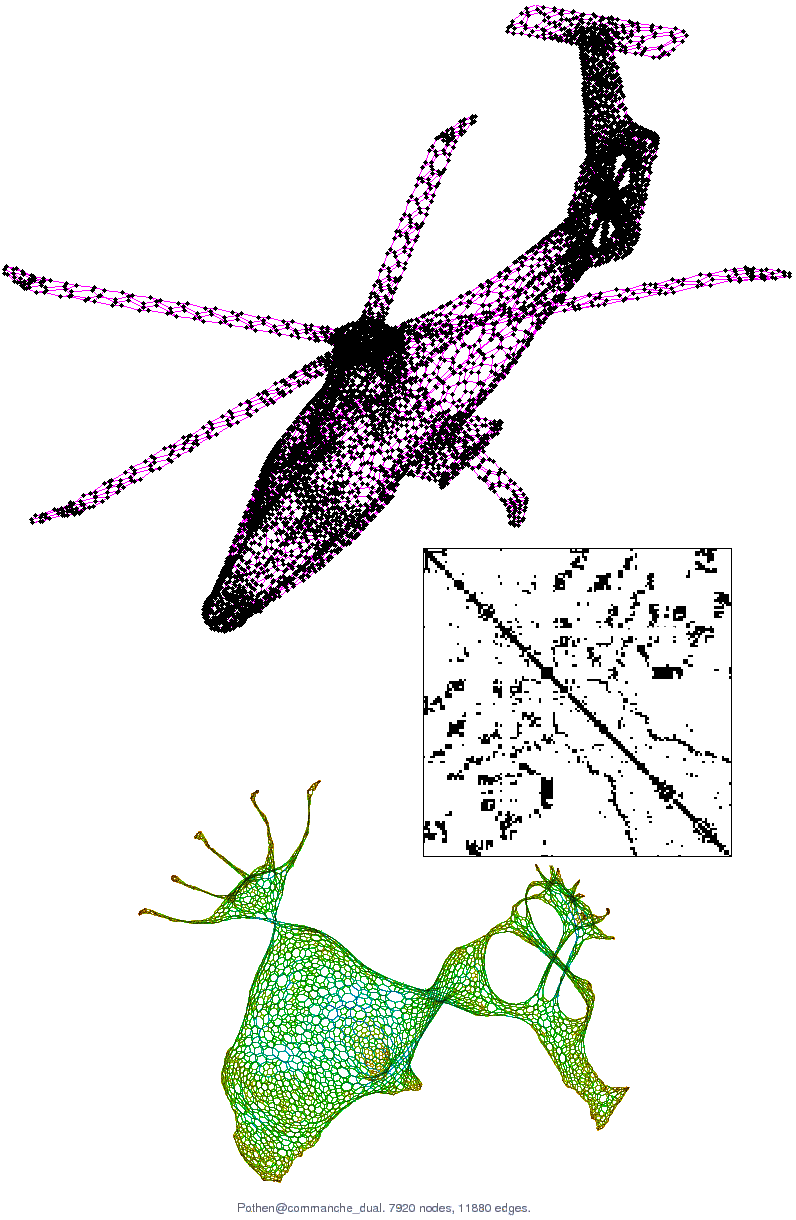
\includegraphics[width=1.0\textwidth]{./images/commanche/commanche}
	\caption{3D neorientovaný graf ve tvaru helikoptéry, jeho reprezentace v řídké matici a výsledek simulace}
	\label{fig:commanche}
\end{figure}

Řídké matice jsou používané ve velké škále oblastí \cite{sparsesw}, například výpočty diferenciálních rovnic, Google page rank, 3D grafika, statistika, těžení z dat, kryptografie a další.

% Použití řídkých matic najdeme 2D/3D grafice, simulaci fyzikálních jevů ať už řešení úloh proudění tekutin, elektrické či meteorologické, statistice, počítání pageranku % a další.
% TODO přeložit: computational fluid dynamics, finite-element methods, statistics, time/frequency 
% domain circuit simulation, dynamic and static modeling of chemical processes, 
% cryptography, magneto-hydrodynamics, electrical power systems, differential
% equations, quantum mechanics, structural mechanics (buildings, ships, aircraft,
% human body parts...), heat transfer, MRI reconstructions, vibroacoustics, linear 
% and non-linear optimization, financial portfolio optimization, semiconductor 
% process simulation, economic modeling, oil reservoir modeling, astrophysics, 
% crack propagation,  Google page rank, 3D computer vision, cell phone tower 
% placement, tomography, multibody simulation, model reduction, nano-technology, 
% acoustic radiation, density functional theory, quadratic assignment, elastic 
% properties of crystals, natural language processing, DNA electrophoresis, ... 

\section{Použití násobení matic}

Násobení maticí může znázorňovat nějakou transformaci jednoho stavu do druhého. Největší uplatnění řídkých matic je tedy v simulaci jevů, například fyzikálních, biologických, chemických, ekonomických a dalších. 

Jako příklad simulace můžeme uvést metodu konečných prvků \cite{4020926}\cite{0967-3334-30-6-S01}.

% http://ocw.mit.edu/courses/materials-science-and-engineering/3-11-mechanics-of-materials-fall-1999/modules/fea.pdf
% http://engineering.dartmouth.edu/~d22888z/documents/EIT_Bath_2011_v2.pdf

Pokud potřebujeme vynásobit jednu matici s více vektory, můžeme vektory složit do matice a provést násobení matice s maticí. To se hodí například v real-time aplikacích.

%psal to tady: http://www.researchgate.net/post/Could_anybody_tell_me_some_models_or_applications_in_which_Sparse_Matrix_Matrix_Products_are_required3
%ale dava to smysl

% \url{http://math.stackexchange.com/questions/116717/can-a-basis-for-a-vector-space-be-made-up-of-matrices-instead-of-vectors}

%\url{http://www.cise.ufl.edu/research/sparse/}

% inverze matic: Matrix multiplication and matrix inversion ItA


\section{Matice}

Matice \textbf{A} typu ($m$, $n$) je $m n$ uspořádaných prvků z množiny $\mathbf{R}$. O prvku $a_{r,s} \in \mathbf{R}, r \in \{1,2,\hdots,m\},s \in \{1,2,\hdots,n\}$ říkáme, že je na r-tém řádku a~s-tém sloupci matice \textbf{A}. Matici \textbf{A} zapisujeme do řádků a~sloupců takto:
\begin{align}
\mathbf{A}=\begin{pmatrix}
a_{1,1} & a_{1,2} & \cdots & a_{1,n} \\
a_{2,1} & a_{2,2} & \cdots & a_{2,n} \\
\vdots  & \vdots  & \ddots & \vdots  \\
a_{m,1} & a_{m,2} & \cdots & a_{m,n}
\end{pmatrix}
\end{align}

Matici \textbf{M} typu ($m$, $n$), kde všechny její prvky jsou rovny nule, nazýváme \textit{nulovou maticí.}

O~matici typu ($m$, $n$) budeme říkat, že je $m$~široká a~$n$~vysoká. Pokud o~matici řekneme že má velikost $n$, myslíme tím, že je typu ($n$, $n$).

\section{Vektor}

Matici \textbf{V} typu (1, n) nazveme vektorem.

\section{Definice násobení matice maticí}
\label{defmmm}

Buď \textbf{A} matice typu ($m$,$n$) s prvky $a_{i,j}$ a \textbf{B} matice typu ($n$,$p$) s prvky $b_{j,k}$. Definujeme součin matic $\mathbf{A} \cdot \mathbf{B}$ jako matici \textbf{C} typu ($m$,$p$) s prvky $c_{i,k}$ které vypočteme jako:

\begin{align}
c_{row,col}=\sum_{k=1}^{N} a_{row,k} \cdot b_{k,col}
\end{align}

Výsledek součinu matic se nezmění, pokud matice doplníme o~libovolný počet nulových řádků a~nebo sloupců. Této vlastnosti můžeme využít pro získání potřebných rozměrů:

\begin{enumerate}
  \item Při násobení matice A typu ($m$,$n$) s maticí B typu ($o$,$p$), kde $ n \neq o $.
  \item Pokud potřebujeme matice stejné velikosti.
  \item Pokud potřebujeme matice určité velikosti, například $ 2^{ \mathbf{N}} $.
\end{enumerate}

Násobení matice vektorem je pouze případem násobení matice typu ($m$,$n$) s maticí typu ($1$,$n$).

\section{Složitosti}

K označení složitostí, ať již časových nebo prostorových (paměťových) používáme \bigO-notaci, která označuje množinu funkcí, asymptoticky rostoucí řádově stejně rychle nebo rychleji.
\begin{align}
\bigO(g(n)) = \left\{ f(n) : \exists c \in R^+ \exists n_0 \in N \forall n \geq n_0 : 0 \leq f(n) \leq cg(n) \right\}
\end{align}
\bigO\texttt{ }notací budeme popisovat nejhorší možný případ. Obdobně $\Theta$ značí funkce rostoucí stejně rychle a $\Omega$ stejně rychle nebo pomaleji.

% IntroductionToAlgoritms 3.1 asymptotic notations 43-97 (1217, 1222).

Pro výpočet složitostí rekurzivních algoritmů používáme mistrovskou metodu \cite{Cormen:2001:IA:580470}. Pokud $a \geq 1, b > 0$ jsou konstanty a $f(n)$ je funkce o jedné proměnné, tak rekurence

\begin{align}
t(n) = at(n/b)+f(n)
\end{align}

má asymptotickou složitost:

\begin{enumerate}
  \item Pro $f(n) = \bigO(n^{log_b{a - \epsilon}})$, kde $\epsilon > 0$ je konstanta platí, že $t(n)=\Theta(n^{log_b{a}})$.
  \item Pro $f(n) = \Theta(n^{log_b{a}})$ platí, že $t(n)=\Theta(n^{log_b{a}}log{n})$.
  \item Pro $f(n) = \Omega(n^{log_b{a + \epsilon}})$, kde $\epsilon > 0$ je konstanta a $af(n/b) \leq cf(n)$ pro konstantu $c < 1$ a $\forall n\geq n_0$, tak platí, že $t(n)=\Theta(f(n))$.
\end{enumerate}

\section{Řídké matice}

Matice, které obsahují velké množství nulových prvků, nazýváme řídké. Nebudeme přesně uvádět, kolik procent z celkového počtu prvků musí být nulových, abychom matici nazývali řídkou. Stejně jako řídkou matici můžeme uložit do formátu pro husté matice, můžeme hustou matici uložit do formátu pro řídké matice.

Řídkost matice budeme vyjadřovat pomocí $nnz$ (Number of NonZero elements), tedy počtem nenulových prvků z celkových $mn$, pro matici A typu ($m$, $n$).

%\section{Typy řídkých matic}
%TODO: typy ridkych matic (pasova, atd, pattern, real)

% \section{Numerická stabilita}

% TODO: numerická stabilita obecne (viz strassen)

% \section{Optimalizace kódu}

% Dnešní překladače umí velice dobře optimalizovat vygenerovaný kód. Pokusy o nějaké mikrooptimalizace program spíše zpomalí.

% Je vhodné používat funkce standartních knihoven, protože bývají optimalizované přímo v assembleru.

% TODO: priklady, zdroje

% \subsection{Rozděl a panuj}
% divide, conquer, combine

% \subsection{Rozbalování cyklů}

% \subsection{AoS -> SoA}

% \subsection{Loop tiling}

% TODO: \url{https://edux.fit.cvut.cz/courses/BI-EIA/_media/lectures/kompilator.pdf}

%-----------------------------------------------------------------------------
%-----------------------------------------------------------------------------
%-----------------------------------------------------------------------------

\chapter{Algoritmy násobení matic}
\label{algo}

V této kapitole představíme některé základní a pokročilejší algoritmy pro násobení matic. Základní algoritmy mají stejnou asymptotickou složitost $\bigO(n^3)$ a liší se pouze přístupem k prvkům, což je důležité pro řídké formáty. Pokročilejší algoritmy jsou sice asymptoticky rychlejší, ale přinášejí nevýhodu ve formě numerické stability a velké skryté konstanty.

\subsection{Pseudokódy}

Pseudokódy v této práci jsou ve stylu syntaxe jazyka Fortran, ale budou představovat zápis jazyka C99. Pro pole platí, že jsou indexovaná od nuly a for cyklus \texttt{for i $\gets$ 0 to 10} bude iterovat od nultého do devátého prvku včetně.

\section{Podle definice}

Základním algoritmem násobení dvou matic je podle definice \ref{defmmm}. Ve třech for cyklech postupně  vybíráme řádky matice A, sloupce matice B a v N krocích násobíme. N je jak šířka matice A, tak i výška matice B.

\begin{algorithm}[H]
	\caption{Násobení matic podle definice}\label{mmm-by-definiton}
	\begin{algorithmic}[1]
		\Procedure{MMM-definition}{$A,B,C$}\Comment{A,B,C jsou matice}
\For{\texttt{$row\gets0$\TO$A.height$}}\Comment{řádky}
	\For{\texttt{$col\gets0$\TO$B.width$}}\Comment{sloupce}
		\State \texttt{$sum \gets 0;$}
		\For{\texttt{$i\gets0$\TO$A.height$}}
			\State \texttt{$sum $ += $ A[row][i] * B[i][col];$}
		\EndFor
		\State \texttt{$C[row][col] \gets sum;$}
	\EndFor
\EndFor
		\EndProcedure
	\end{algorithmic}
\end{algorithm}

Z pseudokódu je vidět, že ve dvou for cyklech provádíme $N$ násobení a $N$ sčítání. Asymptotická složitost je tedy $\bigO(n^2(n + n))$ = $\bigO(n^3)$. V ukázkových výpočtech je násobení pouze $N-1$ krát, to proto, že neuvádíme přičítání k nule (řádek 6).

%%%%%%%%%%%%%%%%%%%%%%%%%%%%%%%%%%%%%%%%%%%%%%%%%%%%%%%%%%%%%%%%%%%%%%%%%%%%%%%%%%%%

\section{Násobení transponovanou maticí}

Pokud nám formát uložení matice nedovolí procházet prvky po sloupcích, je řešením druhou matici transponovat. Poté můžeme násobit řádky matice A s řádky transponované matice B.

\begin{algorithm}[H]
	\caption{Násobení transponovanou maticí}\label{mmm-transpose}
	\begin{algorithmic}[1]
		\Procedure{MMM-transpose}{$A,B,C$}\Comment{A,B,C jsou matice}
\State \texttt{$B \gets transpose(B)$}
\For{\texttt{$rowA\gets0$\TO$A.height$}}\Comment{řádky}
	\For{\texttt{$rowB\gets0$\TO$B.height$}}\Comment{sloupce}
		\State \texttt{$sum \gets 0;$}
		\For{\texttt{$i\gets0$\TO$A.height$}}
			\State \texttt{$sum $ += $ A[rowA][i] * B[rowB][i];$}
		\EndFor
		\State \texttt{$C[rowA][rowB] \gets sum;$}
	\EndFor
\EndFor
		\EndProcedure
	\end{algorithmic}
\end{algorithm}

Podobný algoritmus můžeme použít i~pokud nám formát nedovolí procházet prvky po řádcích, ale pouze po sloupcích. Například v této práci neuvedený Compressed Sparse Columns.

%XXX: Pro matice musí platit, že výška matice A musí být stejná jako výška matice B. (FIXME: je to opravdu tak?)

%%%%%%%%%%%%%%%%%%%%%%%%%%%%%%%%%%%%%%%%%%%%%%%%%%%%%%%%%%%%%%%%%%%%%%%%%%%%%%%%%%%%

\section{Násobení po řádcích}

Další možností, jak násobit dvě matice, kde nám formát uložení nedovolí procházet po sloupcích, je procházet současně řádky matice A i B a přičítat jednotlivé součiny na správné místo ve výsledné matici C.

Nevýhodou tohoto řešení je velký počet náhodných přístupů do pole C. Protože k~prvkům přičítáme, tedy načítáme a sčítáme, je potřeba před samotným násobením nastavit všechny prvky matice C na hodnotu nula.

%tohle neplati: Matice musí být stejně široké i vysoké.

\begin{algorithm}[H]
	\caption{Násobení po řádcích}\label{mmm-by-rows}
	\begin{algorithmic}[1]
		\Procedure{\texttt{MMM-by-rows}}{\texttt{A, B, C}}\Comment{A,B,C jsou matice}
\For{\texttt{r $\gets$ 0\TO A.height}}\Comment{řádky matice A i B}
	\For{\texttt{cA $\gets$ 0\TO A.width}}\Comment{sloupce matice A}
		\For{\texttt{c $\gets$ 0\TO B.width}}\Comment{sloupce matice B}
			\State \texttt{C[r][cA] += A[r][cA] * B[r][cB];}
		\EndFor
	\EndFor
\EndFor
		\EndProcedure
	\end{algorithmic}
\end{algorithm}

%%%%%%%%%%%%%%%%%%%%%%%%%%%%%%%%%%%%%%%%%%%%%%%%%%%%%%%%%%%%%%%%%%%%%%%%%%%%%%%%%%%%

\section{Rekurzivní násobení}

Pro matice A i B o stejné velikosti $ {2^\mathbf{N}} $ můžeme použít rekurzivní přístup, tedy programovací techniku rozděl a panuj, kdy rozdělíme větší problémy na menší podproblémy.

Každou z matic rozdělíme na čtvrtiny a jednotlivé podmatice násobíme algoritmem podle definice, tedy jako matice o velikosti dva.

\label{RecMul}
\label{2x2MMM}
\begin{align}
\begin{pmatrix}
 a & b \\
 c & d
\end{pmatrix} \cdot \begin{pmatrix}
 e & f \\
 g & h
\end{pmatrix} = \begin{pmatrix}
 ae+bg & af+bh \\
 ce+dg & cf+dh
\end{pmatrix}
\end{align}

Tento postup opakujeme, dokud velikostí podmatic nenarazíme na práh, tedy hodnotu, při které opustíme rekurzivní algoritmus a použijeme algoritmus lineární. V ukázkovém pseudokódu dělíme podmatice až na velikost prahu jedna, podmatice tedy obsahují pouze jeden prvek.

\begin{algorithm}[H]
	\caption{Rekurzivní násobení}\label{mmm-recursive}
	\begin{algorithmic}[1]
		\Procedure{MMM-recursive}{$A,B,C,ay,ax,by,bx,cy,cx,n$}
		\If{$n = 1$}
			\State \texttt{$C[cy][cx]\gets C[cy][cx] + A[ay][ax] \cdot B[by][bx];$}
			\State \texttt{$return;$}
		\EndIf
		\ForAll{\texttt{$r \in \{ 0, n/2 \}$}}
			\ForAll{\texttt{$c \in \{ 0, n/2 \}$}}
				\ForAll{\texttt{$i \in \{ 0, n/2 \}$}}
					\State \texttt{MMM-recursive$(A,B,C,ay+i,ax+r,by+c,bx+i,cy+c,cx+r,n/2);$}
				\EndFor
			\EndFor
		\EndFor
		\EndProcedure
	\end{algorithmic}
\end{algorithm}

Pro ilustraci jako příklad uvádíme výpočet horního levého prvku v násobení dvou matic o velikosti $ 2^{2} $. Pro větší přehlednost značíme prvky malým písmem z názvu matice a indexy o jejich pozicích.

\begin{align}
\begin{pmatrix}
a_{1,1} & a_{1,2} & a_{1,3} & a_{1,4} \\
a_{2,1} & a_{2,2} & a_{2,3} & a_{2,4} \\
a_{3,1} & a_{3,2} & a_{3,3} & a_{3,4} \\
a_{4,1} & a_{4,2} & a_{4,3} & a_{4,4}
\end{pmatrix} \cdot \begin{pmatrix}
b_{1,1} & b_{1,2} & b_{1,3} & b_{1,4} \\
b_{2,1} & b_{2,2} & b_{2,3} & b_{2,4} \\
b_{3,1} & b_{3,2} & b_{3,3} & b_{3,4} \\
b_{4,1} & b_{4,2} & b_{4,3} & b_{4,4}
\end{pmatrix} = \notag\\
\begin{pmatrix}
%----------------------------------------
\begin{pmatrix}
 a_{1,1} & a_{1,2} \\
 a_{2,1} & a_{2,2} \\
\end{pmatrix} \cdot
\begin{pmatrix}
 b_{1,1} & b_{1,2} \\
 b_{2,1} & b_{2,2} \\
\end{pmatrix} + 
\begin{pmatrix}
 a_{1,3} & a_{1,4} \\
 a_{2,3} & a_{2,4} \\
\end{pmatrix} \cdot 
\begin{pmatrix}
 b_{3,1} & b_{3,2} \\
 b_{4,1} & b_{4,2} \\
\end{pmatrix} &
\hdots \\
\hdots & \hdots
\end{pmatrix} = \notag\\
\begin{pmatrix}
%----------------------------------------
\begin{pmatrix}
 a_{1,1} b_{1,1}+a_{1,2} b_{2,1} & \hdots \\
 \hdots & \hdots
\end{pmatrix} + 
\begin{pmatrix}
 a_{1,3} b_{3,1}+a_{1,4} b_{4,1} & \hdots \\
 \hdots & \hdots
\end{pmatrix} &
\hdots \notag\\
\hdots & \hdots
\end{pmatrix} = \notag\\
\begin{pmatrix}
\begin{pmatrix}
 a_{1,1} b_{1,1}+a_{1,2} b_{2,1}+a_{1,3} b_{3,1}+a_{1,4} b_{4,1} & \hdots \\
\hdots & \hdots
\end{pmatrix} &
\hdots \\\hdots & \hdots
\end{pmatrix} \notag
\end{align}

Asymptotická složitost je samozřejmě stejná jako u algoritmu podle definice. Asymptotickou složitost rekurzivního algoritmu můžeme spočítat pomocí mistrovské metody.

\[ T(n) = \left\{ 
  \begin{array}{l l}
    \Theta(1) & \quad \text{if $n$ = 1}\\
    8T(n/2) + \Theta(1) & \quad \text{if $n$ > 1}
  \end{array} \right.\]

Protože platí, že $a=8, b=2, r=\log_{2} 8, n^r=n^{\log_{2} 8}=n^3=\Omega(1)$, tak asymptotická složitost podle mistrovské metody je \texttt{MMM-recursive}(n) = $\bigO(n^3)$.

Kvůli režii rekurzivního dělení v praxi nezmenšujeme podmatice až na velikost jedna. Vhodný práh velikosti podmatice je například takový, co se vejde do L1 cache.

%%%%%%%%%%%%%%%%%%%%%%%%%%%%%%%%%%%%%%%%%%%%%%%%%%%%%%%%%%%%%%%%%%%%%%%%%%%%%%%%%%%%%%%%%%%%%%%%%%%%%%%%%%%%%%%%%%%%%%%%%%%%%%%%
\section{Strassenův algoritmus} %%%%%%%%%%%%%%%%%%%%%%%%%%%%%%%%%%%%%%%%%%%%%%%%%%%%%%%%%%%%%%%%%%%%%%%%%%%%%%%%%%%%%%%%%%%%%%%%

V roce 1969 Volker Strassen v časopise Numerische Mathematik publikoval článek \cite{GEMnO}, ve kterém jako první představil algoritmus násobení dvou matic s menší asymptotickou složitostí než algoritmus podle definice, tedy $O(n^3)$.

Algoritmus je založen na myšlence, že sčítání je operace méně náročnější než operace násobení. Respektive dvě matice umíme sečíst nebo odečíst se složitostí $\bigO(n^2)$, ale vynásobit se složitostí $\bigO(n^3)$.

Volker Strassen tedy využil jisté symetrie \cite{StrNat} v násobení dvou matic $A$ a $B$ o velikosti dva a výslednou matici $C$ seskládal pomocí sedmi pomocných matic. Obrázek \ref{fig:StrVis} ukazuje, z čeho se pomocné matice skládají a jak jsou do výsledné matice seskládány. V ilustračních maticích o velikosti čtyři ukazujeme, které sčítance pomocná matice do výsledku přičítá a které odečítá. 

\begin{figure}[H]\centering
	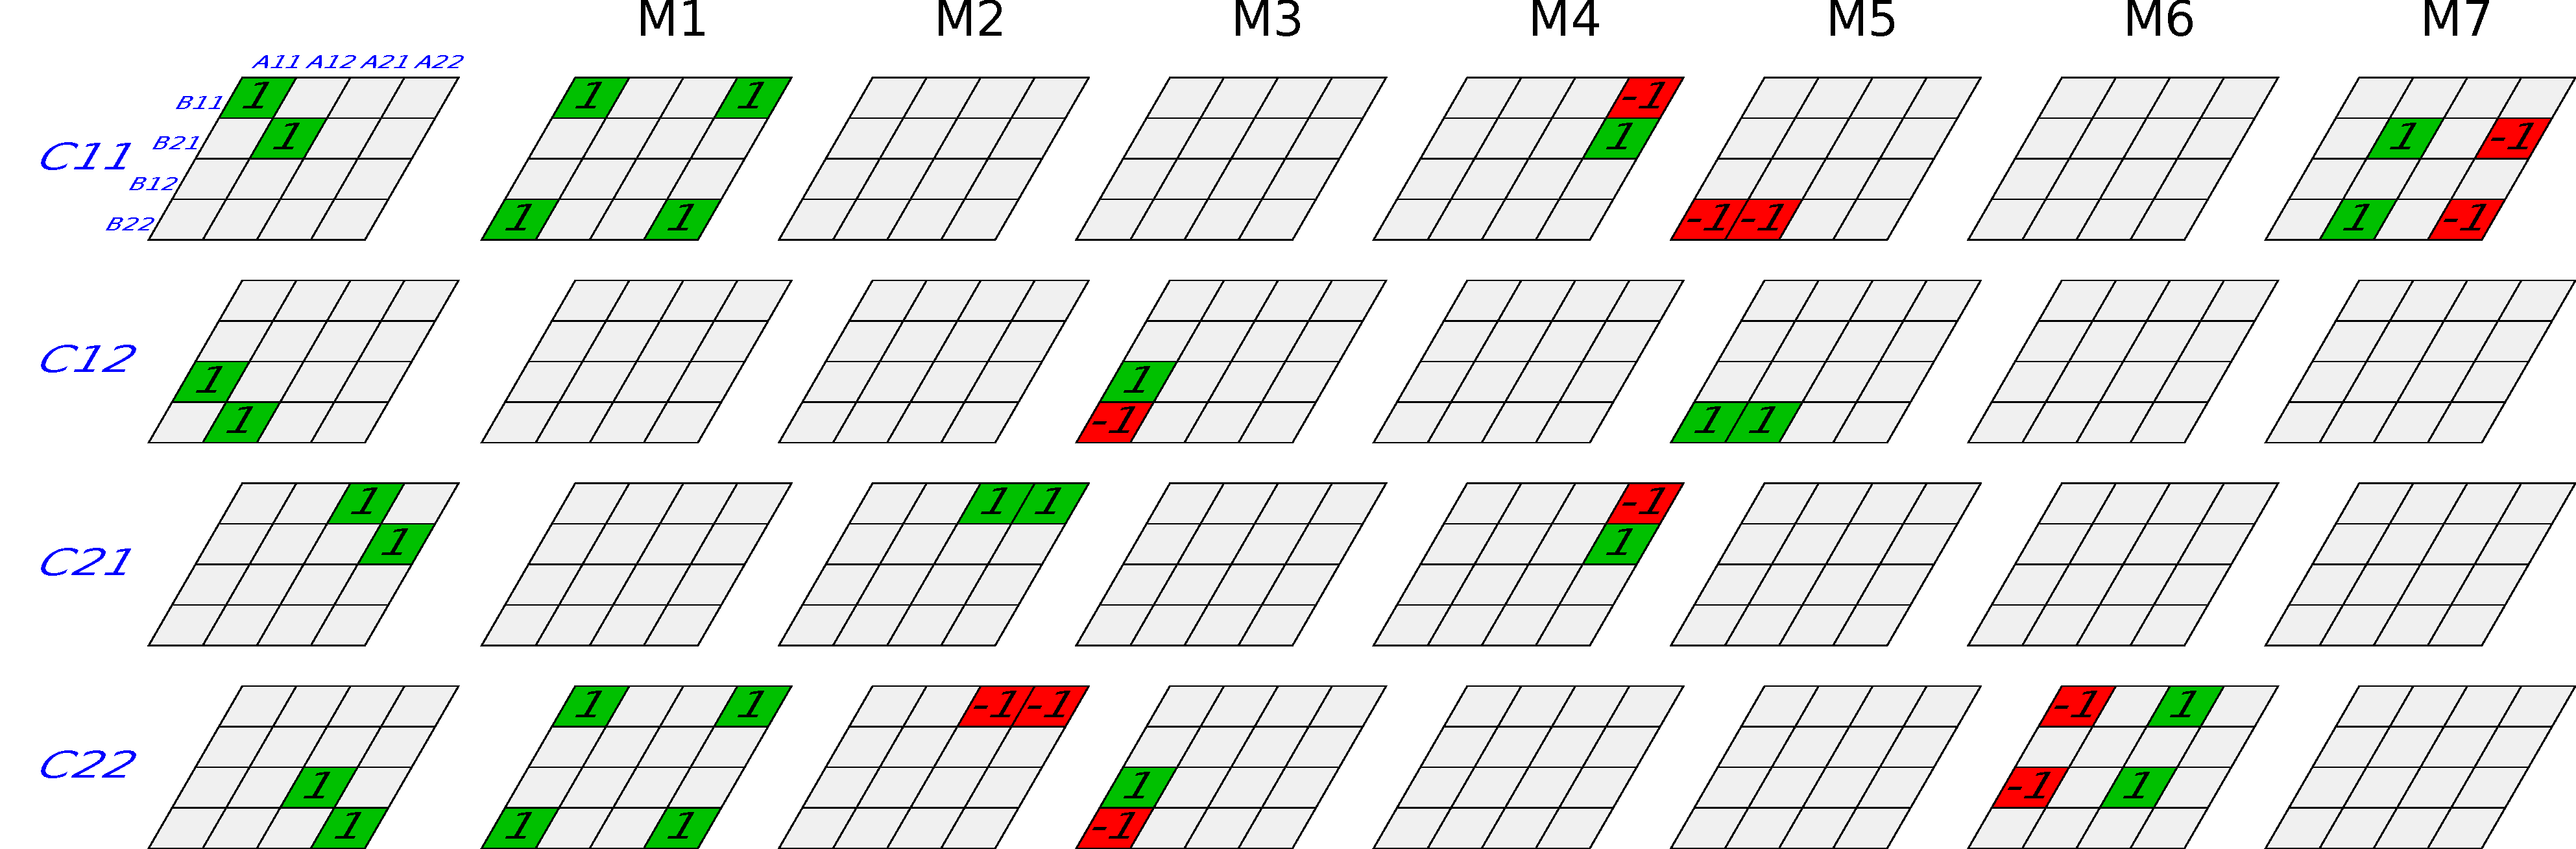
\includegraphics[width=\textwidth]{./images/strassen}
	\caption{Strassenův algoritmus \cite{strassenimage}}
	\label{fig:StrVis}
\end{figure}

Zápis Strassenova algoritmu vypadá následovně:	

\begin{align}
A \cdot B = \begin{pmatrix}
 A_{1,1} & A_{1,2} \\
 A_{2,1} & A_{2,2} \\
\end{pmatrix} \cdot \begin{pmatrix}
 B_{1,1} & B_{1,2} \\
 B_{2,1} & B_{2,2} \\
\end{pmatrix} \notag\\
M_{1} = (A_{1,1} + A_{2,2}) \cdot (B_{1,1} + B_{2,2}) \notag\\
M_{2} = (A_{2,1} + A_{2,2}) \cdot B_{1,1} \notag\\
M_{3} = A_{1,1} \cdot (B_{1,2} - B_{2,2}) \notag\\
M_{4} = A_{2,2} \cdot (B_{2,1} - B_{1,1}) \notag\\
M_{5} = (A_{1,1} + A_{1,2}) \cdot B_{2,2} \notag\\
M_{6} = (A_{2,1} - A_{1,1}) \cdot (B_{1,1} + B_{1,2}) \notag\\
M_{7} = (A_{1,2} - A_{2,2}) \cdot (B_{2,1} + B_{2,2}) \notag\\
C = \begin{pmatrix}
 M_{1} + M_{4} - M_{5} + M_{7} & M_{3} + M_{5} \\
 M_{2} + M_{4} & M_{1} - M_{2} + M_{3} + M_{6}
\end{pmatrix}
\end{align}

V pseudokódu používáme procedury \texttt{offset-add}, respektive \texttt{offset-sub}. Slouží ke sčítání, respektive odečítání bloku prvků o velikosti n v maticích od nějakého offsetu \texttt{y} a \texttt{x}. Parametry obou funkcí jsou: \texttt{offset-*}$(A,B,C,ay,ax,by,bx,cy,cx,n)$. 

\begin{algorithm}[H]
	\caption{Strassenův algoritmus}\label{mmm-strassen}
	\begin{algorithmic}[1]
		\Procedure{MMM-strassen}{$A,B,C,ay,ax,by,bx,cy,cx,n$}
		\If{$n = 1$}
			\State \texttt{$C[cy][cx]\gets C[cy][cx] + A[ay][ax] \cdot B[by][bx];$}
			\State \texttt{$return;$}
		\EndIf
  		\State \texttt{$h \gets n/2;$} \Comment{čtvrtina}
  		\State \texttt{$m[9] \gets $init-matrices$(9, h);$} \Comment{devět pomocných matic}
 % 	
	\State \texttt{offset-add$(a, a, m[8], ay, ax, ay + h, ax + h, 0, 0, h);$} \Comment{M1}
	\State \texttt{offset-add$(b, b, m[9], by, bx, by + h, bx + h, 0, 0, h);$}
	\State \texttt{MMM-strassen$(m[8], m[9], m[1], 0, 0, 0, 0, 0, 0, h);$}
%	
	\State \texttt{offset-add$(a, a, m[8], ay + h, ax, ay + h, ax + h, 0, 0, h);$} \Comment{M2}
	\State \texttt{MMM-strassen$(m[8], b, m[2], 0, 0, bx, by, 0, 0, h);$}
%	
	\State \texttt{offset-sub$(b, b, m[8], by, bx + h, by + h, bx + h, 0, 0, h);$} \Comment{M3}
	\State \texttt{MMM-strassen$(a, m[8], m[3], ay, ax, 0, 0, 0, 0, h);$}
%	
	\State \texttt{offset-sub$(b, b, m[8], by + h, bx, by, bx, 0, 0, h);$} \Comment{M4}
	\State \texttt{MMM-strassen$(a, m[8], m[4], ay + h, ax + h, 0, 0, 0, 0, h);$}
%	
	\State \texttt{offset-add$(a, a, m[8], ay, ax, ay, ax + h, 0, 0, h);$} \Comment{M5}
	\State \texttt{MMM-strassen$(m[8], b, m[5], 0, 0, by + h, bx + h, 0, 0, h);$}
%	
	\State \texttt{offset-sub$(a, a, m[8], ay + h, ax, ay, ax, 0, 0, h);$} \Comment{M6}
	\State \texttt{offset-add$(b, b, m[9], by, bx, by, bx + h, 0, 0, h);$}
	\State \texttt{MMM-strassen$(m[8], m[9], m[6], 0, 0, 0, 0, 0, 0, h);$}
%	
	\State \texttt{offset-sub$(a, a, m[8], ay, ax + h, ay + h, ax + h, 0, 0, h);$} \Comment{M7}
	\State \texttt{offset-add$(b, b, m[9], by + h, bx, by + h, bx + h, 0, 0, h);$}
	\State \texttt{MMM-strassen$(m[8], m[9], m[7], 0, 0, 0, 0, 0, 0, h);$}
%	
	\State \texttt{offset-add$(m[1], m[4], m[8], 0, 0, 0, 0, 0, 0, h);$} \Comment{c1,1}
	\State \texttt{offset-sub$(m[8], m[5], m[8], 0, 0, 0, 0, 0, 0, h);$}
	\State \texttt{offset-add$(m[8], m[7], c, 0, 0, 0, 0, cy, cx, h);$}
%	
	\State \texttt{offset-add$(m[3], m[5], c, 0, 0, 0, 0, cy, cx + h, h);$} \Comment{c1,2}
%	
	\State \texttt{offset-add$(m[2], m[4], c, 0, 0, 0, 0, cy + h, cx, h);$} \Comment{c2,1}
%	
	\State \texttt{offset-sub$(m[1], m[2], m[8], 0, 0, 0, 0, 0, 0, h);$} \Comment{c2,2}
	\State \texttt{offset-add$(m[8], m[3], m[8], 0, 0, 0, 0, 0, 0, h);$}
	\State \texttt{offset-add$(m[8], m[6], c, 0, 0, 0, 0, cy + h, cx + h, h);$}		
		\EndProcedure
	\end{algorithmic}
\end{algorithm}

Výpočet asymptotické složitosti provedeme podobně jako u \texttt{MMM-recursive}, tedy mistrovskou metodou. 

V každém kroku rekurze počítáme $\Theta(n^2)$ operací na vytvoření pomocných matic.

\[ T(n) = \left\{ 
  \begin{array}{l l}
    \Theta(1) & \quad \text{if $n$ = 1}\\
    7T(n/2) + \Theta(n^2) & \quad \text{if $n$ > 1}
  \end{array} \right.\]

Protože platí, že $a=7, b=2, r=\log_{2} 7, n^r=n^{\log_{2} 7}=\Omega(n^2)$, tak asymptotická složitost podle mistrovské metody je \texttt{MMM-strassen}(n) = $\bigO(n^{\log_{2} 7}) \approx \bigO(n^{2.8})$.

Stejně jako v předešlém algoritmu i zde demonstrujeme výpočet levého horního prvku matice z násobení dvou matic o velikosti dva. Místo parametrické matice použijeme konkrétní desetinná čísla, abychom ukázali numerickou stabilitu Strassenova algoritmu. Pro ukázku budeme uvažovat počítač, který u čísel ukládá pouze pět cifer, znaménko a desetinnou čárku.	

Pomocí algoritmu podle definice by takový počítač vypočítal součin dvou matic následovně:

\begin{align}
\begin{pmatrix}
 30.234 & 0.5678 \\
 0.9123 & 10.456
\end{pmatrix} \cdot \begin{pmatrix}
 0.8912 & 0.3456 \\
 0.7891 & 9.999 \\
\end{pmatrix} = \begin{pmatrix}
 27.392 & \hdots \\
 \hdots & \hdots
\end{pmatrix} \notag
\end{align}

Správný výsledek je $30.234 \times 0.8912 + 0.5678 \times 0.7891 = 26.9445408 + 0.44805098 = 27.39259178$.

Nyní výpočet provedeme pomocí Strassenova algoritmu:

\begin{align}
\begin{pmatrix}
 30.234 & 0.5678 \\
 0.9123 & 10.456
\end{pmatrix} \cdot \begin{pmatrix}
 0.8912 & 0.3456 \\
 0.7891 & 9.999
\end{pmatrix} \notag\\
M_{1} = (30.234 + 10.456) \cdot (0.8912 + 9.999) = 443.12  \notag\\
\hdots \notag\\
M_{4} = 10.456 \cdot (0.7891 - 0.8912) = -1.067 \notag\\
M_{5} = (30.234 + 0.5678) \cdot 9.999 = 307.98 \notag\\
\hdots \notag\\
M_{7} = (0.5678 - 10.456) \cdot (0.7891 + 9.999) = -106.67 \notag\\
 \begin{pmatrix}
 M_{1} + M_{4} - M_{5} + M_{7} & \hdots \\
 \hdots & \hdots
\end{pmatrix} = \begin{pmatrix}
 27.403 & \hdots \\
 \hdots & \hdots
\end{pmatrix} \notag
\end{align}

% zdroj http://math.nist.gov/MatrixMarket/data/Harwell-Boeing/oilgen/orsirr_1.html

Jak můžeme vidět, zatímco u algoritmu podle definice jsme pouze ztratili desetinnou přesnost, výsledek Strassenova algoritmu se lišil už v prvním desetinném čísle. 

Pro reálnou představu stability Strassenova algoritmu jsme provedli experiment, ve kterém jsme vynásobili dvě stejné matice (matice orsirr\_1, oříznuta na velikost 1024) algoritmem podle definice a Strassenovým algoritmem s různými prahy a sečetli všechny rozdíly mezi výsledky. Násobení probíhalo ve dvojité desetinné přesnosti, tedy v datovém typu \texttt{double} jazyka C99. Z grafu \ref{fig:StrassenStability} je vidět exponenciální závislost mezi velikostí prahu a celkovou chybou.

\begin{figure}[H]\centering
	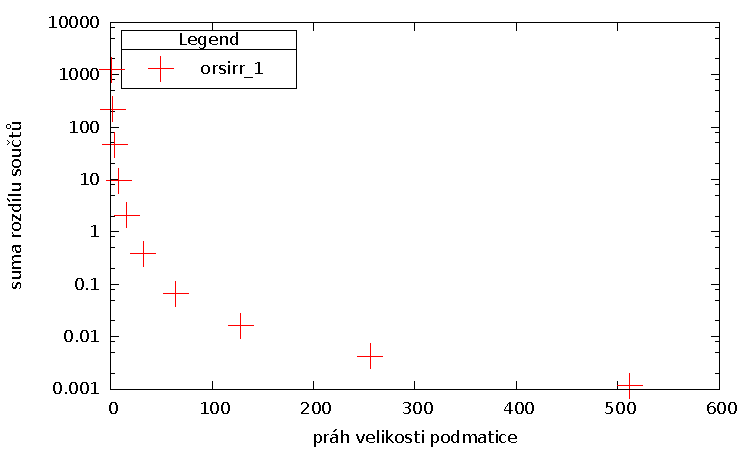
\includegraphics[width=\textwidth]{./images/strassen_stability}
	\caption{Ukázka numerické stability Strassenova algoritmu}
	\label{fig:StrassenStability}
\end{figure}

Strassenův algoritmus lze ještě vylepšit. Algoritmům na stejném principu se říká Strassen-like \cite{DBLP:journals/iacr/CenkH13}. Pro sedm operací násobení je možné snížit počet sčítání a odečítání. Pro jednoduchost zde uvádíme pouze originální algoritmus.

\section{Rychlé algoritmy}

Potom, co Strassen ukázal, že existují rychlejší algoritmy než $\bigO(n^3)$, ještě rychlejší algoritmy než ten jeho na sebe nenechaly dlouho čekat. Složitost násobení matic pro jednoduchost označíme jako $\bigO(n^\omega)$.

Nejpomalejší algoritmus s $\omega=3$ je podle definice. Strassenův algoritmus se sedmi násobeními má $\omega\approx2.807354$. Jeden z nejrychlejších algoritmů je algoritmus Virginie Williamsové \cite{DBLP:conf/stoc/Williams12}\cite{BreakigCWB}, pro který je $\omega<2.3727$. 

Hranicí nejlepší možné složitosti může být $\omega=2$, protože každý prvek z matice musíme nějak započítat. Existují z velké části podložené domněnky na základě teorie grup \cite{complexityMM}, že $\omega=2$ skutečně platí, ale přímý důkaz ještě neexistuje.

\section{Algoritmus podle definice upravený pro řídké matice}

Pokud násobíme řídké matice $A$ a $B$ o velikosti $N$, můžeme vynechat násobení takových dvou prvků, z nichž je alespoň jeden nulový. Označme $nnzr_{M,i}$ jako počet nenulových prvků v i-tém řádku matice M a $nnzc_{M,i}$ jako počet nenulových prvků v i-tém sloupci matice M. Protože násobíme každý řádek s každým sloupcem, bude celkový počet operací násobení dán vzorcem:

\begin{figure}[htb]\label{csrmmm}
\begin{align}
\sum_{i=1}^{n} nnzr_{A,i} \cdot nnzc_{B,i}
\end{align}
\end{figure}

Složitost tohoto algoritmu pro násobení dvou matic $A$ a $B$ o velikosti $n$ tedy můžeme vyjádřit jako $O(mn)$, kde $m = max(nnz(A),nnz(B)$. Pro husté matice bez jediného nulového prvku samozřejmě platí, že $m=n^2$. Nutno podotknout, že $O(mn)$ je nejhorší případ, kdy se všechny nenulové prvky matice $A$ budou násobit se všemi nenulovými prvky matice $B$.

Pro reálnou představu demonstrujeme násobení dvou stejných matic. Opět se jedná o dvě matice orsirr\_1 \cite{mtxors}. Matice orsirr\_1 má velikost $n=1030$ a~$m=6858$ nnz. Rozmístění nnz před respektive po vynásobení ukazují obrázky \ref{fig:befOrsirr1} respektive \ref{fig:aftOrsirr1}.


\begin{figure}[htb]
	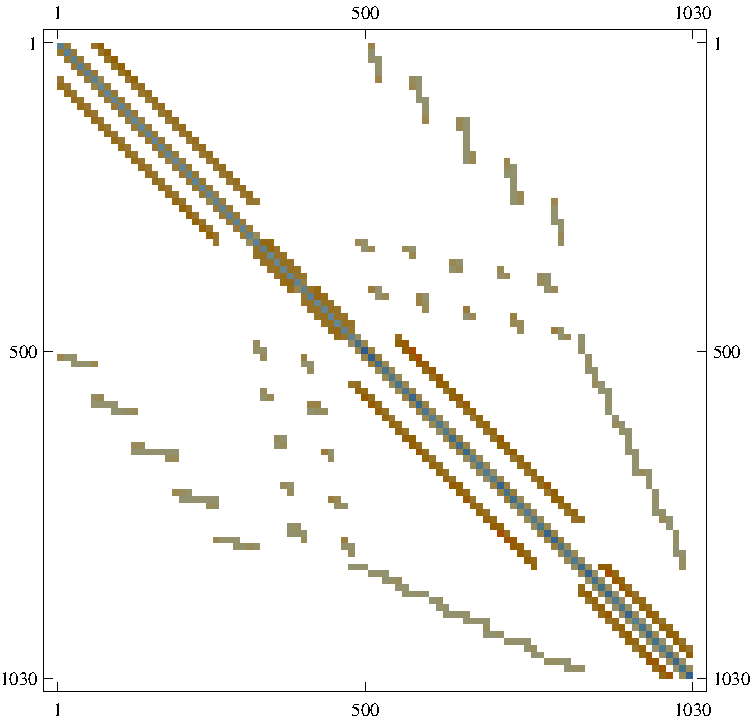
\includegraphics[width=1.0\textwidth]{./images/orsirr_1_orig}
	\caption{Matice orsirr\_1 před vynásobením}
	\label{fig:befOrsirr1}
\end{figure}

\begin{figure}[htb]
	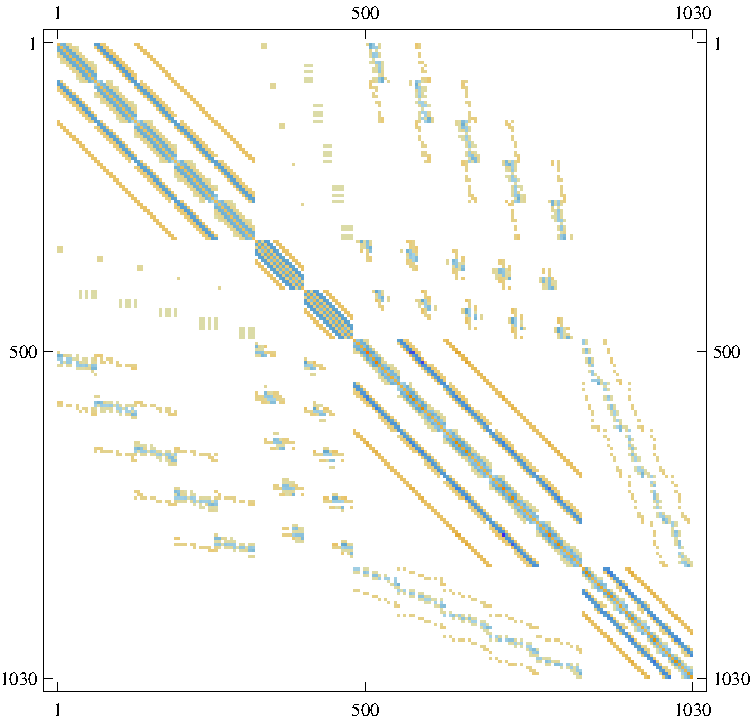
\includegraphics[width=1.0\textwidth]{./images/orsirr_1_mul}
	\caption{Matice orsirr\_1 po vynásobením sama se sebou}
	\label{fig:aftOrsirr1}
\end{figure}

Kdyby nastal nejhorší možný případ, počet operací násobení při použití algoritmu podle definice pro řídké matice by byl $1030 \times 6858 = 7.063740\e{6}$. Pro tento případ ovšem stačí $4.6976\e{4}$ operací násobení. Oproti nejhoršímu možnému případu nastalo $7.063740\e{6} - 4.6976\e{4} = 7.016764\e{6}$ situací, kdy jeden ze dvou prvků byl nulový a operace násobení nemusela být provedena. Při násobení algoritmem podle definice pro husté matice by v $1.092680024\e{9}$ případech operace násobení nemusela být provedena, protože alespoň jeden ze dvou prvků by byl nula. Po vynásobení matice orsirr\_1 sama se sebou stoupl její počet nnz z $6858$ na $23532$. V tomto případě to bylo především z důvodu, že všechny prvky z diagonály matice jsou nenulové, každý prvek se tedy započítá.

\label{fast-sparse}
\section{Rychlé násobení řídkých matic}

Strassenův algoritmus $\omega\approx2.807354$ od $nnz<n^{1.8}$ a algoritmus Virginie Williamsové $\omega<2.3727$ od $nnz<n^{1.37}$ jsou asymptoticky stejně rychlé jako algoritmus podle definice upravený pro řídké matice $\bigO(mn)$. Například pro $n=1000$ je tato hranice pro Strassenův algoritmus $251189$ (40 \%) nnz a pro algoritmus Virginie Williamsové $12882$ (78 \%) nnz z celkových možných $1000000$ prvků.

Raphael Yuster a Uri Zwick ukázali algoritmus \cite{DBLP:journals/talg/YusterZ05} s asymptotickou složitostí $\bigO(m^{0.7}n^{1.2}+n^{2+o(1))}$, který rozdělí permutace řádků a sloupců na řídké a husté. Řídké permutace násobí algoritmem podle definice v úpravě pro řídké matice $\bigO(mn)$. Husté permutace vynásobí v té době nejznámějším nejrychlejším algoritmem, a to od Dona Coppersmitha a Shmuela Winograda s asymptotickou složitostí $\omega=2.375477$ \cite{DBLP:journals/jsc/CoppersmithW90}.

\section{Další algoritmy pro řídké matice}

Algoritmů násobení řídkých matic je mnoho. Často se odvíjejí od typu řídkých matic a formátu, v jakém jsou uloženy. Příkladem může být formát, ve kterém se ukládají diagonály \cite{diagonalTvrdikSimecek}.


\chapter{Formáty uložení řídkých matic}


Formáty uložení řídkých matic obecně ukládají jednotlivé elementy zvlášť a tedy nemusí ukládat ty nulové. To ale přináší řadu nevýhod. Za prvé se musí ukládat informace o souřadicních jednotliých prvcích. Za druhé, ztrácíme možnost přístupu k prvku na libovolných šouřadnicích v čase $\Theta(1)$, protože prvky nemáme přímo indexované podle jejich umístění v řádku a sloupci.

Protože řídké matice můžeme rozdělit do mnoha kategorií a provádět nad nimi mnoho operací, existuje hodně formátů, jak řídkou matici efektivně uložit a pracovat s ní.

\url{http://www.cs.colostate.edu/~mroberts/toolbox/c++/sparseMatrix/sparse_matrix_compression.html}

\subsection{Modifikace řídké matice}

Formáty uložení řídkých matic můžeme také rozdělit podle toho, zda-li je možné do nich přidávat nebo odebírat prvky.

Při násobení matic $C = A \cdot B$ se matice $A$ ani $B$ nemění. V této práci budeme předpokládat, že matice $C$ bude hustá a formáty umožujícími přidávání nebo odebírání prvků nebudou součástí práce. Stejně tak při násobení matice $A$ vektorem $B$ je výsledek $C$ vektor.

\subsection{Uspořádanost řídké matice}

Dalším kritériem pro rozdělení formátů je uspořádanost nenulových prvků v řídké matici. Pro uspořádané prvky bude efektivnější takový formát, který využije určitý vzor. V řídkých maticích takovým vzorem může být například diagonála, nebo blok prvků. Efektivně lze za vzor považovat i prvky v řádku, nebo ve sloupci.

Uspořádáním může být také symetrie matice, kdy nám stačí uložit pouze polovinu matice. Zpravidla řídké matice bývají symetrické podle hlavní diagonály.

\section{COO - Coordinate list}

Formát COO, česky seznam souřadnic, je základní formát řídkých matic. Ke~každému nenulovému prvku ukládá jeho souřadnice \texttt{y} a \texttt{x}. Implementovat tento formát můžeme například jako tři pole, jedno s hodnotami prvků, druhé s \texttt{y} souřadnicemi a třetí s \texttt{x} souřadnicemi.

Pro ukázku v tomto formátu uložíme matici o velikosti $n=8$ s $nnz=5$ nenulovými prvky.

\begin{align}
\begin{pmatrix}
	0 & 0 & 0 & 0 & 0 & 0 & 0 & 0 \\
	\boldsymbol{1} & \boldsymbol{2} & 0 & 0 & 0 & 0 & 0 & 0 \\
	0 & 0 & 0 & 0 & 0 & 0 & 0 & 0 \\
	0 & 0 & 0 & 0 & 0 & 0 & 0 & 0 \\
	0 & \boldsymbol{3} & 0 & 0 & 0 & 0 & 0 & 0 \\
	0 & 0 & 0 & 0 & 0 & 0 & 0 & 0 \\
	0 & 0 & 0 & 0 & 0 & \boldsymbol{4} & \boldsymbol{5} & 0 \\
	0 & 0 & 0 & 0 & 0 & 0 & 0 & 0 \\	
\end{pmatrix}
\end{align}

\begin{table}[H]
    \begin{tabular}{r|lllll}
    values[5]   & 1 & 2 & 3 & 4 & 5 \\
    y-coords[5] & 1 & 1 & 4 & 7 & 7 \\
    x-coords[5] & 0 & 1 & 1 & 5 & 6 \\
    \end{tabular}
    \caption{Matice uložená ve formátu COO}
\end{table}

Jak můžeme vidět, délka polí je závislá pouze na $nnz$. Pro velké matice s malým počtem neuspořádaných nenulových prvků je tento formát velmi efektivní. Pokud by bylo prvků velké množství, informace o uložení \texttt{y} nebo \texttt{x} souřadnic by byla často redundatní.

Formát COO je velmi jednoduchý a přímočarý. Při procházení jeho prvků nám stačí jedna iterace přes tři stejně dlouhé pole. Tím je tedy například algoritmus násobení řídké matice ve formátu COO s vektorem velmi jednoduchý:

\begin{algorithm}[H]
	\caption{Násobení matice COO s vektorem}\label{coo-mvm}
	\begin{algorithmic}[1]
		\Procedure{COO-MVM}{$COO,V,C$}
		\For{\texttt{$i\gets0$\TO$COO.nnz$}}
			\State \texttt{$V.v[COO.r[i]] \gets V.v[COO.r[i]] + COO.v[i] * V.v[COO.c[i]];$}
		\EndFor
		\EndProcedure
	\end{algorithmic}
\end{algorithm}

\label{alg:coo-mmm}
Při násobení dvou matic ale narazíme na problém. Při této operaci se každý prvek násobí dvakrát. Potřebujeme způsob, jak se v matici vrátit zpátky na určité místo. Takový naivní algoritmus pro násobení dvou COO matic by byl složitý. Museli bychom si pamatovat začátky řádků a neustále kontrolovat, jestli jsme nepřesáhli další řádek. Lepším řešením je dopředu si předpočítat, kde který řádek začíná a končí. Předpočítáme si tedy pole, nazvané $row\_pointers$, o délce $M.height + 1$, obsahující indexy začátků a konců řádek.

Při procháchezní matice se tak v poli s prvky mezi indexy $row\_pointers[i]$ a $row\_pointers[i+1]$ nachází prkvy na řádku $i$. Proto je pole právě o jedna delší než výska matice, abychom mohli určit konec posledního řádku.

\begin{algorithm}[H]
	\caption{Násobení dvou COO matic}\label{coo-mmm}
	\begin{algorithmic}[1]
		\Procedure{COO-MMM}{$A,B,C$}
		\State \texttt{$arp\gets InitArray(A.nnz + 1);$}
		\State \texttt{$brp\gets InitArray(B.nnz + 1);$}
		\For{\texttt{$i\gets0$\TO$A.nnz$}}\Comment{předpočítání prvků v řádcích matice A}
			\State \texttt{$arp[A.r[i]+1] = arp[A.r[i]+1] + 1;$}
		\EndFor
		\For{\texttt{$i\gets0$\TO$A.height$}}
			\State \texttt{$arp[i+1] = arp[i+1] + arp[i];$}
		\EndFor
		\For{\texttt{$i\gets0$\TO$B.nnz$}}\Comment{předpočítání prvků v řádcích matice B}
			\State \texttt{$brp[B.r[i]+1] = brp[B.r[i]+1] + 1;$}
		\EndFor
		\For{\texttt{$i\gets0$\TO$A.height$}}
			\State \texttt{$brp[i+1] = brp[i+1] + brp[i];$}
		\EndFor
		\For{\texttt{$i\gets0$\TO$A.height$}}\Comment{násobení}
			\For{\texttt{$ac\gets arp[i]$\TO$arp[i+1]$}}
				\For{\texttt{$bc\gets brp[A.c[ac]]$\TO$brp[A.c[ac]+1]$}}
					\State \texttt{$C.v[r][A.c[bc]] \gets C.v[r][A.c[bc]] + A.v[ac] * B.v[bc];$}
				\EndFor
			\EndFor
		\EndFor
		\EndProcedure
	\end{algorithmic}
\end{algorithm}

V části s násobením již pole s \texttt{y} souřadnicemi nepotřebujeme. Lepší formát uložení řídkých matic pro násobení by byl takový, který namíto pole s \texttt{y} souřadnicemi obsahuje předpočítané začátky a konce řádků. Takovým formátem je CSR.

%%%%%%%%%%%%%%%%%%%%%%%%%%%%%%%%%%%%%%%%%%%%%%%%%%%%%%%%%%%%%%%%%%%%%%%%%%%%%%
%%%%%%%%%%%%%%%%%%%%%%%%%%%%%%%%%%%%%%%%%%%%%%%%%%%%%%%%%%%%%%%%%%%%%%%%%%%%%%
%%%%%%%%%%%%%%%%%%%%%%%%%%%%%%%%%%%%%%%%%%%%%%%%%%%%%%%%%%%%%%%%%%%%%%%%%%%%%%
%%%%%%%%%%%%%%%%%%%%%%%%%%%%%%%%%%%%%%%%%%%%%%%%%%%%%%%%%%%%%%%%%%%%%%%%%%%%%%
%%%%%%%%%%%%%%%%%%%%%%%%%%%%%%%%%%%%%%%%%%%%%%%%%%%%%%%%%%%%%%%%%%%%%%%%%%%%%%
%%%%%%%%%%%%%%%%%%%%%%%%%%%%%%%%%%%%%%%%%%%%%%%%%%%%%%%%%%%%%%%%%%%%%%%%%%%%%%

\section{CSR - Compressed sparse row}

Problém efektivnosti formátu COO pro větší množství prvků řeší formát CSR, česky komprimované řídké řádky. Formát CSR obsahuje pole $row\_pointers$, které ukládá informace o tom, kolik se v daném řádku nachází prvků. K poli s hodnotami je další pole $col\_indicies$, přiřazující ke každému prvku informaci o sloupci.

\begin{figure}[H]\centering
	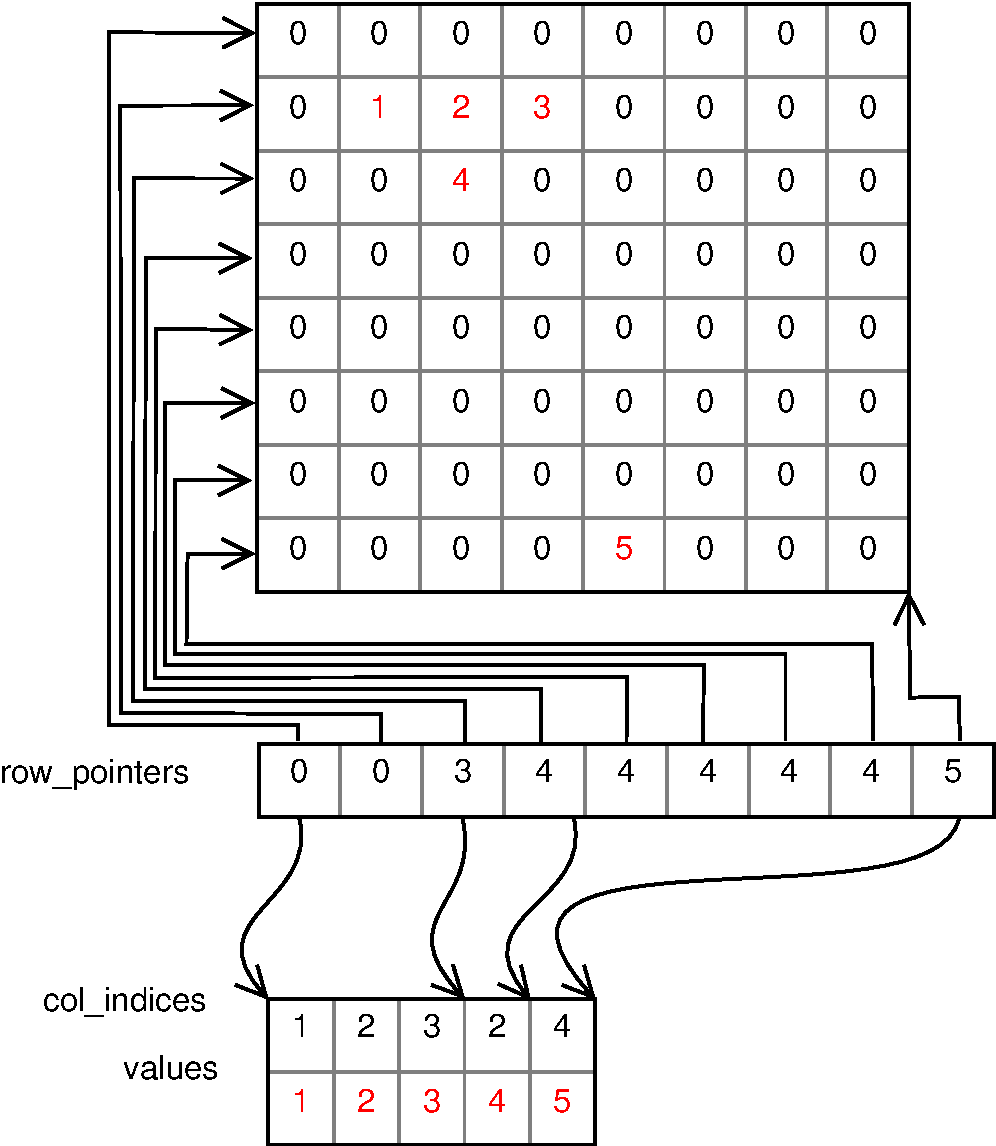
\includegraphics[width=\textwidth]{./images/csr/csr}
	\caption{Matice uložená ve formátu CSR}
	\label{fig:CSR}
\end{figure}

Jak je vidět z ilustrace \ref{fig:CSR}, řádek s více prvky je uložen efektivně. Díky prázdným řádkům se nezdá pole $row\_pointers$ rozumně využité.

Při násobení matice CSR s vektorem potřebujeme o jeden for cyklus více než v případě násobení matice COO s vektorem. Důvodem je ztráta informace o řádku prvku.

\begin{algorithm}[H]
	\caption{Násobení matice CSR s vektorem}\label{csr-mvm}
	\begin{algorithmic}[1]
		\Procedure{CSR-MVM}{$CSR,V,C$}
		\For{\texttt{$i\gets0$\TO$CSR.h$}}
			\For{\texttt{$ci\gets CSR.rp[i]$\TO$CSR.rp[i + 1]$}}
				\State \texttt{$C.v[r] \gets C.v[r] + CSR.v[ci] * V.v[A.ci[ci]];$}
			\EndFor
		\EndFor
		\EndProcedure
	\end{algorithmic}
\end{algorithm}

Násobení dvou CSR matic je stejné jak v případě násobení dvou COO matic popsaném v sekci \nameref{alg:coo-mmm}. Jediný rozdíl je, že předpočíné začátky a konce řádků jsou součástí formátu.

\label{alg:csr-mmm}
\begin{algorithm}[H]
	\caption{Násobení dvou CSR matic}\label{csr-mmm}
	\begin{algorithmic}[1]
		\Procedure{CSR-MMM}{$A,B,C$}
		\For{\texttt{$i\gets0$\TO$A.height$}}\Comment{násobení}
			\For{\texttt{$ac\gets A.rp[i]$\TO$A.rp[i+1]$}}
				\For{\texttt{$bc\gets B.rp[A.ci[ac]]$\TO$B.rp[A.ci[ac]+1]$}}
					\State \texttt{$C.v[r][B.ci[bc]] \gets C.v[r][B.ci[bc]] + A.v[ac] * B.v[bc];$}
				\EndFor
			\EndFor
		\EndFor
		\EndProcedure
	\end{algorithmic}
\end{algorithm}

Existuje varianta tohoto formátu, nazvaná CSC - compressed sparse columns, která místo ukládání řádku ukládá sloupce.


\section{BSR - Block Sparse Row}

Jako formát CSR využívá uložení prvků v řádku, formát BSR ještě navíc detekuje a ukládá prvky v blocích.

Protože při násobení matic násobíme každý prvek dvakrát, bylo by dobré tyto dvě operace provést co nejdříve, abychom při druhém znovunačtení prvku mohli sáhnout pro prvek do cache. Pokud jsou prkvy procházené po menších blocích, dostaneme se k prvku podruhé dříve, než jej z cache přemaže jiný prvek.

Matici $A$ ve formátu BSR uklákáme, velice podobně jako u formátu CSR, pomocí tří polí a jedné proměnné, která uchovává velikost bloku. Tuto proměnnou nazveme ji $block\_size$. Matici rozdělíme do bloků Pole $col\_indices$ označuje sloupec, ve kterém se blok nachází. Sloupcem rozumíme $A.width / A.block\_size$.

\begin{figure}[H]\centering
	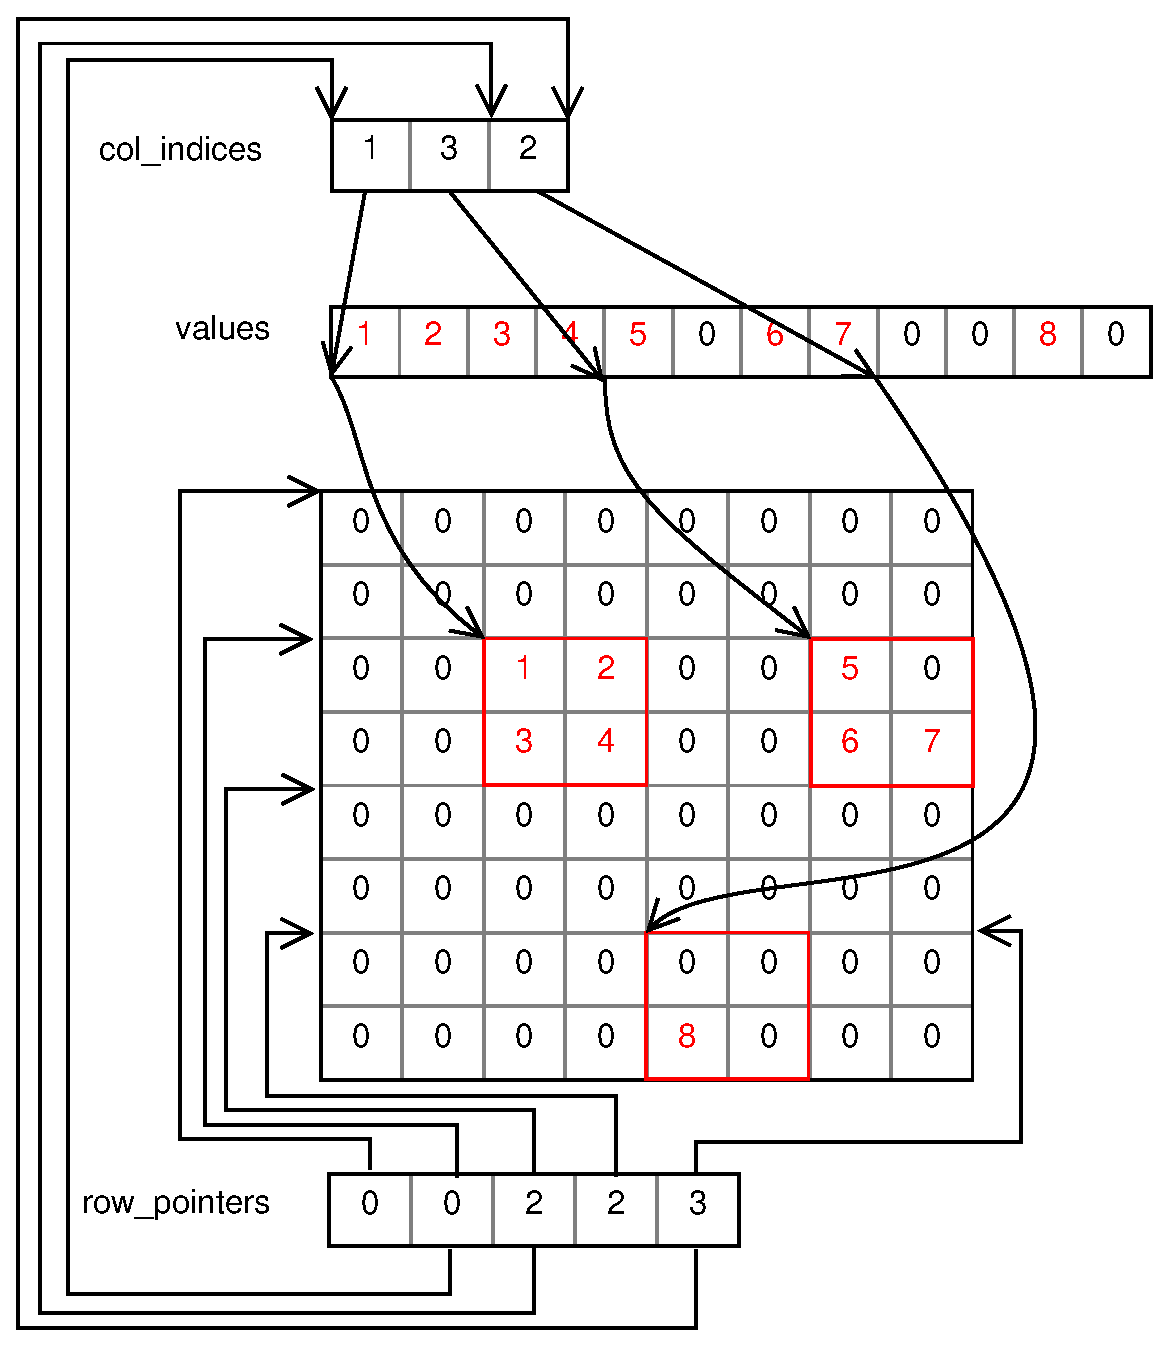
\includegraphics[width=\textwidth]{./images/bsr/bsr}
	\caption{Matice uložená ve formátu BSR}
	\label{fig:CSR}
\end{figure}


Pokud vezmeme algoritmus násobení dvou CSR matic a místo prvků násobíme bloky, vznikne nám algoritmus pro násobení dvou BSR matric. Za povšimnutí stojí větší počet for cyklů s menším rozsahem iterace. To nám v nejvnitřnejších cyklech dovoluje lépe využívat cache. Jedná se tedy o přístup podobný loop tilingu.

\label{alg:bsr-mmm}
\begin{algorithm}[H]
	\caption{Násobení dvou BSR matic}\label{bsr-mmm}
	\begin{algorithmic}[1]
		\Procedure{BSR-MMM}{$A,B,C$}
		\State \texttt{$bs\gets A.block\_size;$}
		\For{\texttt{$i\gets0$\TO$A.height / bs$}}
			\For{\texttt{$ac\gets A.rp[i]$\TO$A.rp[i+1]$}}
				\For{\texttt{$bc\gets B.rp[A.ci[ac]]$\TO$B.rp[A.ci[ac]+1]$}}
					\For{\texttt{$l\gets0$\TO$A.bs$}}\Comment{násobení bloku}
						\For{\texttt{$m\gets0$\TO$bs$}}
							\For{\texttt{$n\gets0$\TO$bs$}}
								\State \texttt{$C.v[(i * bs) + l][(B.ci[bc] * bs) + m]$ += \\
									$ A.v[ac * (bs * bs) + (l * bs) + n] *$
									$ B.v[bc * (bs * bs) + (n * bs) + m];$}
							\EndFor
						\EndFor
					\EndFor
				\EndFor
			\EndFor
		\EndFor
		\EndProcedure
	\end{algorithmic}
\end{algorithm}



\url{http://docs.scipy.org/doc/scipy-0.13.0/reference/generated/scipy.sparse.bsr_matrix.html}
\url{https://software.intel.com/sites/products/documentation/doclib/mkl_sa/11/mklman/GUID-9FCEB1C4-670D-4738-81D2-F378013412B0.htm}



\section{Quadtree}

\section{?}

TODO: tady jsem chtel spocictat kdy  se vyplati mit ridkou matici, ale lepsi bude tabulka. Pokud například uložíme matici o rozměrech 100x100 v dvojté přestnosti, bude zabírat \texttt{M x N x sizeof(double) = 100 x 100 x 8 = 80000B = 80kB}. Pokud zvolíme řídký formát matice, kde ke každému elementu uložíme i jeho x a y souřadnici, tak do 80kB uložíme \texttt{80000 / (sizeof(int)+sizeof(int)+sizeof(double)) = 80000/16= 5000} elementů. Pokud matice obsahuje více jak 50  \% nulových elementů, vyplatí se nám ji uložit do řídkého formátu.

%-----------------------------------------------------------------------------

\chapter{Modifikace formátu quadtree}

je to samostatnej bod v zadani tak by to mohla byt cela chapter

TODO: popsat nevyhody quadtree a obrazkama ukazat jak to udelat lip

neco jako quadtree loop unrolling


\chapter{Analýza a návrh}

V této kapitole představíme některé známé systémy, které umí pracovat s řídkými maticemi. Popíšeme možnosti implementace a zvolené řešení.

Pokud potřebujeme rychle vynásobit dvě malé matice, můžeme použít obecný nástroj, se kterým se snadno pracuje. Čím je ale nástroj obecnější, tím spíš bude pomalejší. Některé nástroje jsou ale specificky optimalizované a i přes jejich obecnost mají dobrou výkonnost. Maximální efektivnosti dosáhneme, pokud co nejvíce využijeme hardware a náš program bude řešit konkrétní úkol. 

\section{Software pro práci s řídkými maticemi}

\subsection{SciPy.sparse}

SciPy je knihovna skriptovacího jazyka Python \cite{Python}. Obsahuje modul pro základní práci s řídkými maticemi nazvaný sparse \cite{scipy}. Samotné výpočty nad řídkými maticemi jsou v této knihovně z důvodu rychlosti napsány v jazyce C++.

\subsection{Boost}

Pro práci s řídkými maticemi v jazyce C++ je možné použít knihovnu uBLAS \cite{ublas} ze sady knihoven Boost\cite{boost}. Knihovna uBLAS obsahuje algoritmy pro řešení základních úkolů z lineární algebry. Protože je kód napsaný pomocí C++ šablon, je vygenerovaný kód výkonný.

\subsection{ATLAS}

ATLAS \cite{atlas} je v překladu zkratkou pro automatické generování vyladěného kódu pro software řešící úlohy z lineární algebry. Tohoto je dosaženo jak pomocí obecných optimalizací kódu, tak optimalizací pro konkrétní architektury.

Podobných projektů je více, konkrétně pro násobení matice s vektorem je to například Sparsity \cite{sparsity} nebo pro násobení matice s maticí je to například PHiPAC \cite{PHiPAC}\cite{bilmes96a}.

\subsection{Wolfram Mathematica}

Wolfram Mathematica \cite{mathematica} je mocný výpočetní software. Práce v tomto software je snadná, interaktivní a přitom dokáže efektivně rozdělovat práci nejen na více procesorových jader, ale také využít grafické karty. Nechybí tedy ani implementace operací pro řídké matice.

V této práci pomocí Wolfram Mathematicy vizualizujeme řídké matice z formátu \texttt{.mtx} \ref{mtxsubsect}. Mathematica umí pracovat i s maticemi v souborech \texttt{.mtx.gz}, tedy komprimovanými soubory. Příkaz pro importování řídké matice a její vizualizaci je \texttt{Import["/var/tmp/matrix.mtx", "Graphics"]}, následné uložení matice lze provést například příkazem \\ \texttt{Export["/var/tmp/matrix.pdf", \%]} \cite{mathematicaMTX}.

\section{Řešení implementace}

Jednou z možných variant bylo pro porovnání všech zvolených formátů byla doimplementovat formát Quadtree, respektive KAT do knihovny SciPy.sparse. Další možností bylo pokračovat v semestrální práci z předmětu Efektivní implementace algoritmů s tématem násobení matic ve formátu CSR.

Protože se v této práci zabýváme pouze vlivem uložení řídké matice pro operaci násobení, rozhodli jsme se vytvořit program pouze pro tuto operaci. Obecná knihovna pro práci s řídkými maticemi, jakým například SciPy.sparse je, nemůže využít některých vlastností matic při jejich násobení. Hlavně zacházení s násobenými maticemi jako s konstantami. Navíc pokud nebudou použity žádné jiné implementace, budou všechny algoritmy stejně optimalizované. Navážeme tedy na semestrální práci. Pro každý formát vytvoříme ve zdrojovém kódu třídu, v níž implementujeme operaci násobení s maticí a násobení s vektorem.


\chapter{Realizace}

\section{Prostředí}

Popsané algoritmy jsme implementovali v jazyce C99[todo: zdroj]. Implementace probíhala v operačním systému Lubuntu[todo: zdroj], v IDE Eclipse CDT[todo: zdroj]. Zdrojový kód byl kompilován pomocí překladače GNU C[todo: zdroj], s optimalizačním přepínačem \texttt{--Ofast}.

K lazení chyb pro práci s pamětí jsme použili nástroj Valgrind[todo: zdroj] s přepínači \texttt{----leak--check=full ----show-reachable=yes}. Běžící program jsme krokovali pomocí nástroje GNU Debugger[todo: zdroj]. Zdrojový kód pro lazení chyb byl kompilován s přepínači \texttt{--Wall --pedantic --Og --ggdb}.

%-----------------------------------------------------------------------------

\section{Design implementace}

Po různých formátech požadujeme stejné operace, proto v programu zavádíme abstraktní matici a jednoduchý objektově orientovaný model \cite{schreiner1994objektorientierte}, kde formáty dědí z virtuální matice. Obrázek \ref{fig:uml} ukazuje jednoduchý návrh tříd v UML.
	
\begin{figure}[htb]
	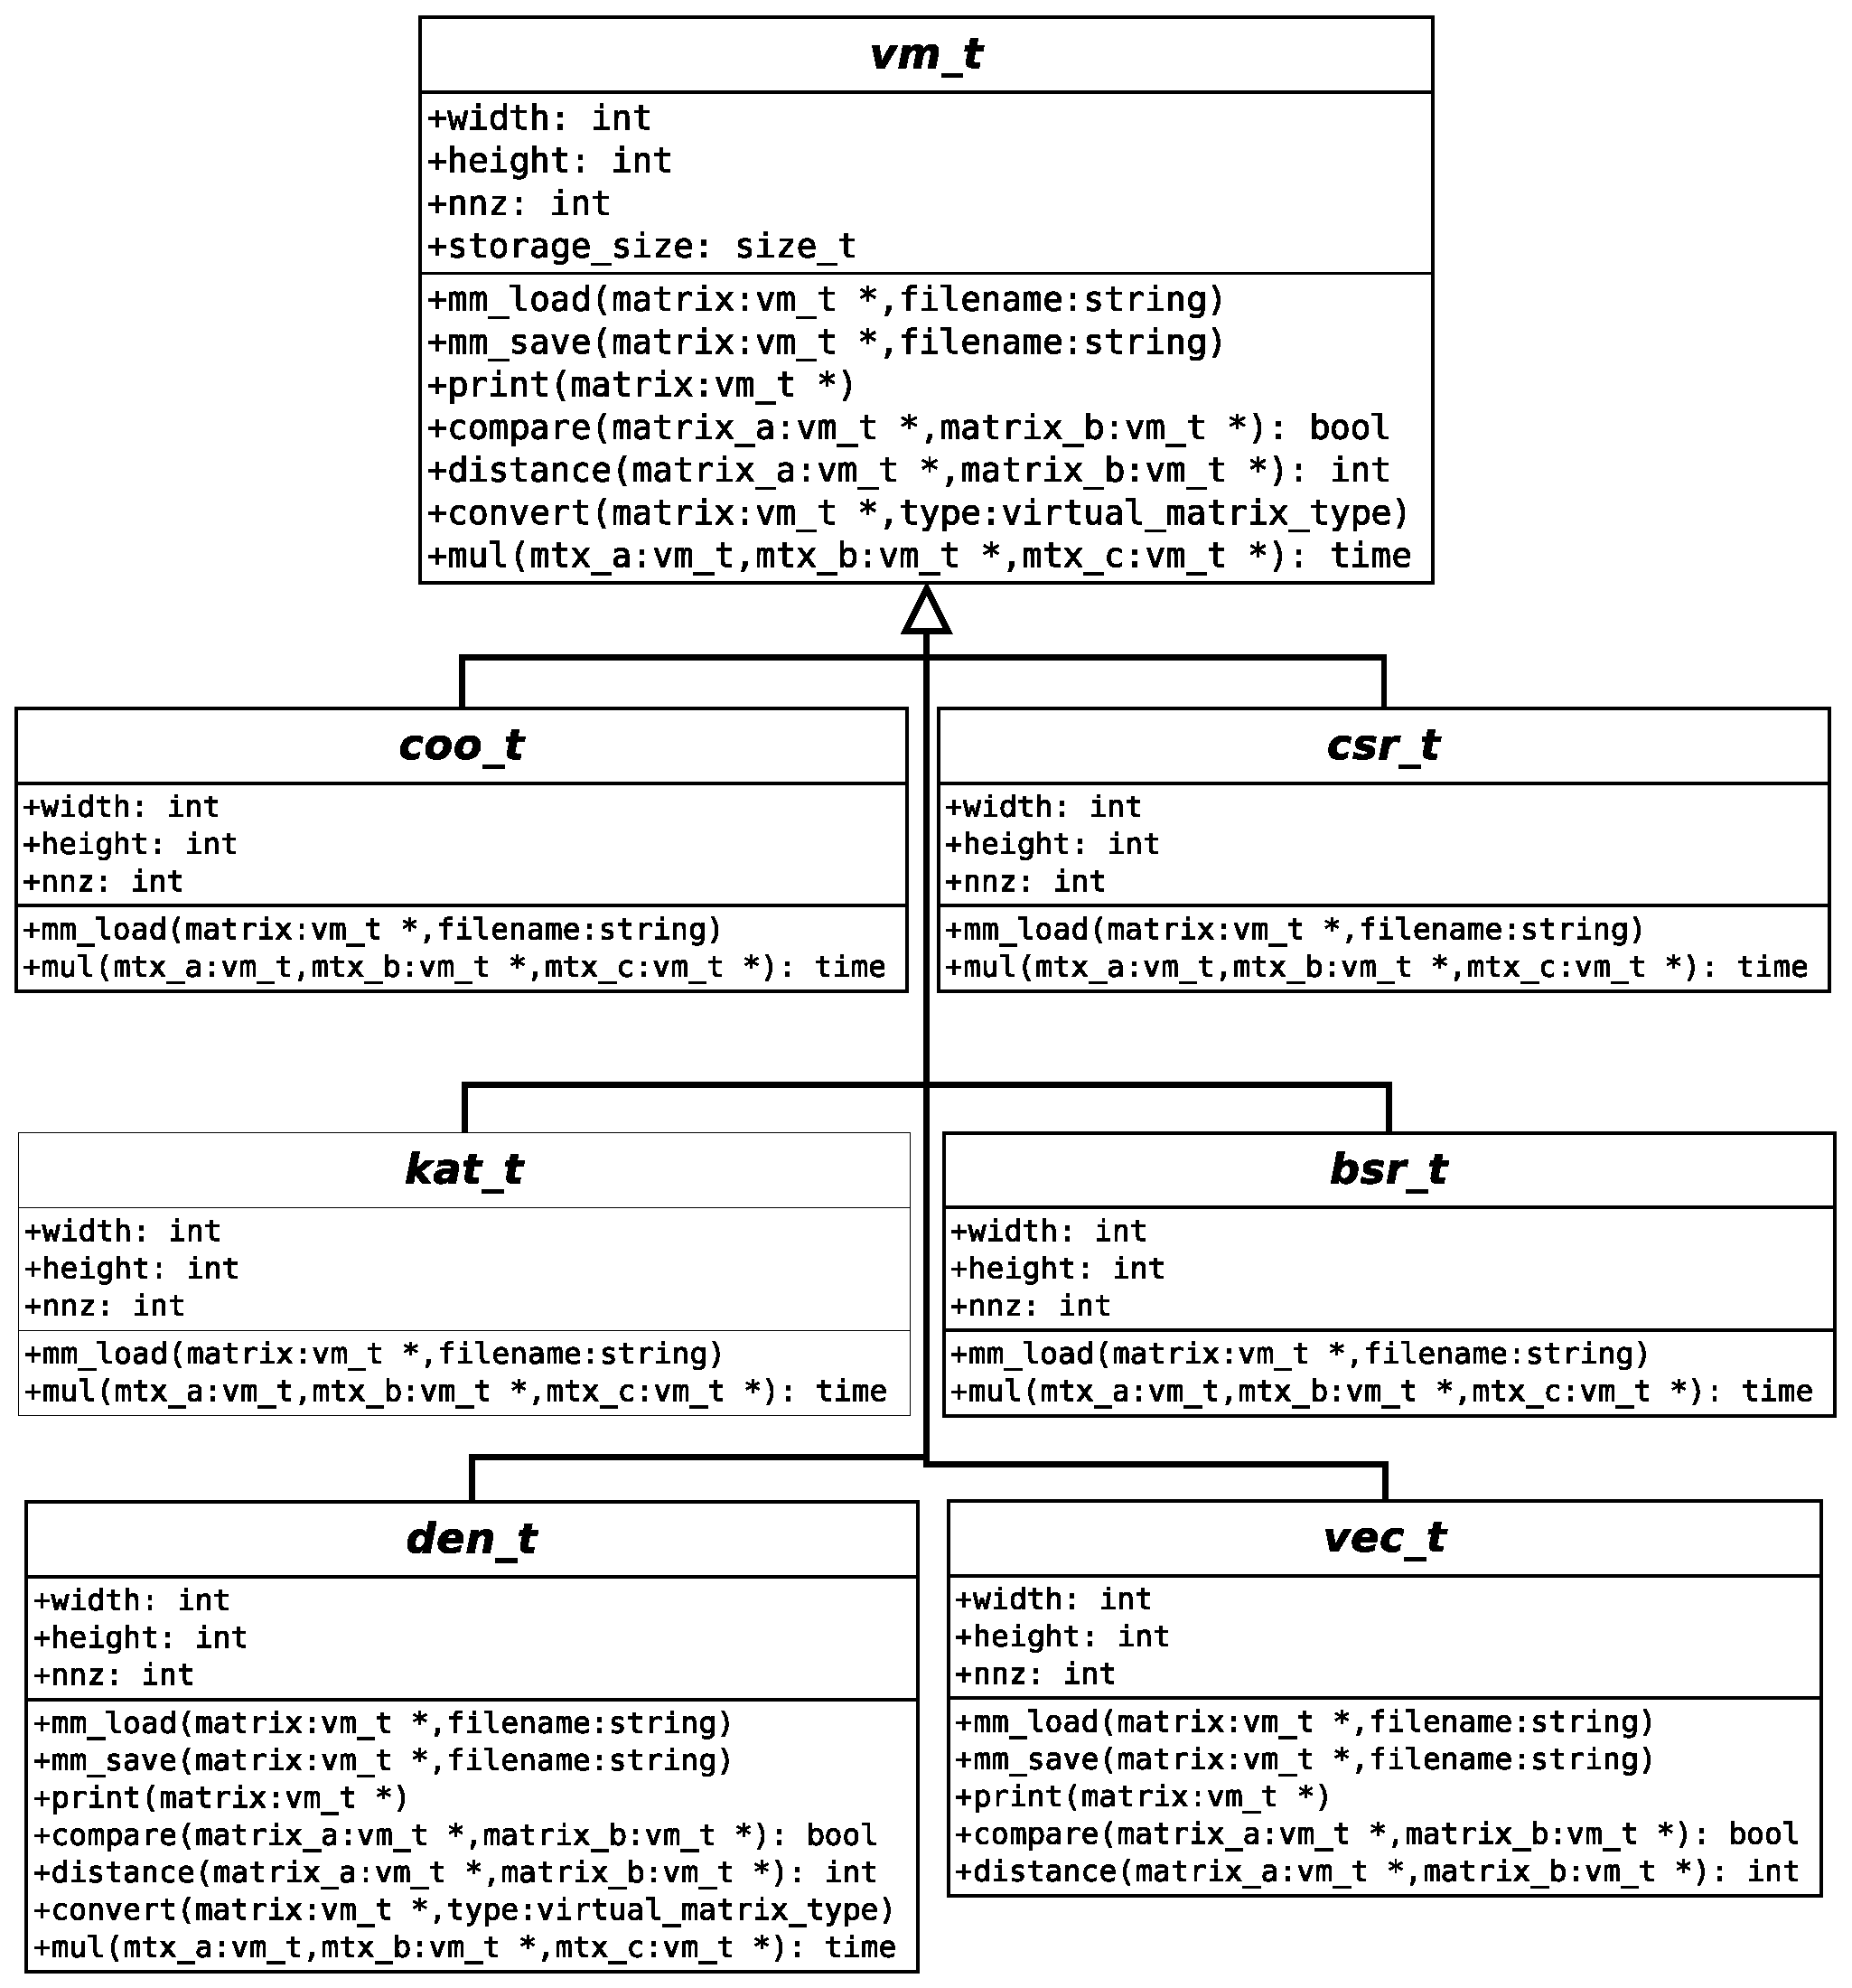
\includegraphics[width=1.0\textwidth]{./images/uml/uml}
	\caption{UML diagram tříd programu}
	\label{fig:uml}
\end{figure}

Program běží v příkazovém řádku bez GUI. Program je jedno-vláknový. Program načte jednu, nebo dvě matice v určitém formátu a vynásobí je. Pomocí přepínačů lze zobrazit, nebo uložit výslednou matici, popřípadě vypsat některé údaje o načtených maticích. Podrobnější popis nastavení programu je v příloze.

%-----------------------------------------------------------------------------

\section{Implementace KAT}

U formátů COO, CSR, BSR je implementace přímočará podle pseudokódů. U implementace KAT máme více možností, proto zde popíšeme naší implementaci.

Jeden z důležitých parametrů je $k$, tedy maximální počet synů vnitřních uzlů. V naší implementaci je tento parametr uložen v konstantě \texttt{KAT.n}, pro připomenutí $KAT.n = sqrt(k)$. Překladač poté cykly, kde iterujeme do této konstanty, rozbalí. Překladači i explicitně sdělujeme, ať cykly rozbalí přes atribut \texttt{\_\_attribute\_\_((optimize("unroll-loops")))}.

V bakalářské práci Rozšíření implementace formátu kvadrantového stromu od Tomáše Karabely[todo: zdroj] je Quadtree implementován jako strom, jehož listy tvoří virtuální matice podobným těm v naší práci. Protože jeho formát byl určený pro algoritmus LU rozklad, jeho virtuální matice musely umět přijímat i další prvky. Protože v naší práci se s formáty uložení řídké matice zachází jako s konstantami, rozhodli jsme se hodnoty prvků a informace v polích \texttt{row\_pointers} a \texttt{col\_indices} uložit mimo listy stromu. V listech se nachází ukazatel do velkého pole na příslušné místo pro daný list. Ušetříme tak práci knihovně libc s mnohonásobným volání funkce \texttt{malloc}

\subsection{Tvoření stromu}

Při tvoření matice v KAT formátu, pro každý prvek procházíme strom a hledáme správný list. Protože výška stromu je daná třemi parametry, tedy velikostí matice $n$, velikostí podmatice $sm\_size$ a počtu větvení uzlu $k$, nejefektivnější využití bude, pokud je $n$ bezezbytku dělitelné $k * sm\_size$. Pokud toto neplatí, rodiče listů budou mít část synů nevyužitých i při uložení husté matice. Protože se prvky do matice načítají po řádcích zleva doprava, je velká pravděpodobnost, že další načtený prvek bude patřit do stejného listu. Z tohoto důvodu si pamatujeme poslední list a pokud prvek patří do něj, vrátíme jej. Algoritmus \ref{kat-create} ukazuje, jakým způsobem vyhledáváme list pro prvek.


\label{alg:kat-create}
\begin{algorithm}[htb]
	\caption{Vyhledání listu pro KAT matici}\label{kat-create}
	\begin{algorithmic}[1]
		\Procedure{KAT-getNode}{KAT, y, x}
		\If{ \{y, x\} $\in$ lastLeaf.area}
			\State \texttt{return lastLeaf;}
		\EndIf
		\State \texttt{tmpNode $\gets$ KAT.root;}
		\State \texttt{blockY $\gets$ 0;}\Comment{výřez matice}
		\State \texttt{blockX $\gets$ 0;}
		\State \texttt{blockS $\gets$ KAT.sm\_size;}
		\\\Comment{až do předposledního vnitřního uzlu traverzujeme podle velikosti KAT.n}
		\While{\texttt{blockS > (KAT.n * KAT.sm\_size)}}
			\State \texttt{nodeY $\gets$ (y - blockY) / (blockS / KAT.n);}
			\State \texttt{nodeX $\gets$ (x - blockX) / (blockS / KAT.n);}
			\State \texttt{tmpNode $\gets$ tmpNode.childs[nodeY][nodeX];}
			\State \texttt{blockY += nodeY * (blockS / KAT.n);}
			\State \texttt{blockX += nodeX * (blockS / KAT.n);}
			\State \texttt{blockS /= KAT.n;}
		\EndWhile
		\\\Comment{do posledního vnitnřního uzlu traverzujeme podle velikosti KAT.sm\_size}
		\State \texttt{nodeY $\gets$ (y - blockY) / KAT.sm\_size;}
		\State \texttt{nodeX $\gets$ (x - blockX) / KAT.sm\_size;}
		\State \texttt{tmpNode $\gets$ tmpNode.childs[nodeY][nodeX];} 	
		\\\Comment{nyní je tmpNode list}
		\State \texttt{tmpNode.y $\gets$ $\lfloor$y / KAT.sm\_size$\rfloor$ * KAT.sm\_size ;}
		\State \texttt{tmpNode.x $\gets$ $\lfloor$x / KAT.sm\_size$\rfloor$ * KAT.sm\_size ;}
		\State \texttt{lastLeaf $\gets$ tmpNode;}
		\State \texttt{return tmpNode;}
		\EndProcedure
	\end{algorithmic}
\end{algorithm}

\subsection{Násobení listů matice KAT}

Protože dovolujeme dva druhy listů, tedy hustý a řídký ve formátu CSR, bylo potřeba implementovat následující algoritmy:

\begin{enumerate}
  \item hustý list $\cdot$ hustý list
  \item hustý list $\cdot$ CSR list
  \item hustý list $\cdot$ vektor
  \item CSR list $\cdot$ hustý list
  \item CSR list $\cdot$ CSR list
  \item CSR list $\cdot$ vektor
\end{enumerate}

Protože tyto algoritmy jsou velice podobné již popsaným algoritmům \ref{algo}, ukážeme zde pouze násobení CSR listu s hustým listem.

\begin{algorithm}[htb]
	\caption{Násobení hustého KAT listu s CSR listem}\label{kat-mmm-den-csr}
	\begin{algorithmic}[1]
		\Procedure{KAT-MMM-DEN-CSR}{ka,kb,na,nb,c}\Comment{ka,kb=KAT matice; na,nb=listy, c = hustá matice}
		\For{\texttt{i $\gets$ 0 \TO ka.sm\_size}}
			\For{\texttt{j $\gets$ na.rp[i]\TO na.rp[i]}}
				\For{\texttt{k $\gets$ 0 \TO ka.sm\_size}}
					\State \texttt{C.v[na.y + i][nb.x + k] += na.v[j] * nb.v[ka.sm\_size * na.ci[j] + j];}
				\EndFor
			\EndFor
		\EndFor
		\EndProcedure
	\end{algorithmic}
\end{algorithm}


%-----------------------------------------------------------------------------

\section{Testování}

Pro ověření správnosti algoritmů je potřeba testovací software. Strategie testování v našem programu spočívá ve výběru testovacích matic, vynásobení v hustém formátu uložení, vynásobení v některém z řídkých formátů uložení a porovnaní výsledků. Tento proces ukazuje algoritmus \ref{testing}.

\begin{algorithm}[htb]
	\caption{Testování}\label{testing}
	\begin{algorithmic}[1]
		\Procedure{\texttt{TestFormats}}{\texttt{PairList, FormatList}}
		\ForAll{\texttt{pair $\in$ PairList}}
				\State \texttt{denseA $\gets$ vm\_load(pair.a, DENSE);}
				\State \texttt{denseB $\gets$ vm\_load(pair.b, DENSE);}
				\State \texttt{denseC $\gets$ vm\_mul(denseA, denseB, denseC);}
			\ForAll{\texttt{format $\in$ FormatList}}		
				\State \texttt{sparseA $\gets$ vm\_load(pair.a, format);}
				\State \texttt{sparseB $\gets$ vm\_load(pair.b, format);}
				\State \texttt{sparseC $\gets$ vm\_mul(sparseA, sparseB, sparseC);}
				\If{ \texttt{vm\_compare(denseC, sparseC) = NOT\_SAME}}
					\State \texttt{print("Error:", pair.a, pair.b, format);}
				\EndIf
			\EndFor
		\EndFor
		\EndProcedure
	\end{algorithmic}
\end{algorithm}

Pro přehled o nefungujících konfiguracích jsme použili testovací framework Cassertion [todo: zdroj].

Při testování jsme i na relativně malých maticích narazili na problém s numerickou stabilitou. Část z testovacích matic má velký desetinný rozvoj a protože čísla jsou v různých formátech násobena v jiném pořadí, dochází k rozdílu mezi výsledky. Při kompilaci programu lze nastavit přesnost výpočtu pomocí typu proměnné pro uchovaní hodnot buď na \texttt{float}, \texttt{double} nebo \texttt{long double}. Při porovnávání dvou matic neporovnáváme hodnoty přímo, ale sledujeme velikost jejich rozdíl. V defaultní konfiguraci je povolená odchylka 0.001, při kompilaci lze změnit. Pokud spustíme testy  pouze s přesností \texttt{float}, část testů selže právě kvůli numerické stabilitě. 

%-----------------------------------------------------------------------------

\section{Práce s formátem MatrixMarket}
\label{MM}

Náš program pracuje s formátem \texttt{.mtx} \ref{mtxsubsect}. Podporujeme více druhů tohoto formátu. Nesymetrický, s banerem \texttt{\%\%MatrixMarket matrix coordinate real symmetric} a symetrický s banerem \texttt{\%\%MatrixMarket matrix coordinate real general}. Místo reálných čísel podporujeme i druh \texttt{pattern}, kdy nenulové prvky nabývají pouze hodnoty jedna.

Přestože náš program neumí pracovat s komprimovanými soubory, v prostředí unixového systému předáváme programu pojmenovanou rouru do které komprimovanou matici rozbalujeme příkazem \texttt{ <(gzip -cd matrix.mtx.gz) }.

\subsection{Generátor řídkých matic}

Generátory z MatrixMarketu běží v internetovém prohlížeči a v jazyce Java. Protože takto není jednoduché matice generovat ve skriptu, abychom při distribuci našeho programu nemuseli přikládat velké testovací matice, implementovali jsme jednoduchý generátor řídkých matic. Parametry předáváme programu informace o výsledné matici a seznam objektů, tedy buď podmatic nebo diagonál, které mají být do matice zahrnuty. Manuál ke generátoru je možné vypsat zavoláním \texttt{./tests/bin/matrix\_generator -h}.    

\begin{algorithm}[htb]
	\caption{Generování řídkých matic}\label{mmm-recursive}
	\begin{algorithmic}[1]
		\Procedure{SparseMatrixGenerator}{$file,width,height,ItemList$}
		\State \texttt{$MtxWrapper \gets InitMtxWrapper();$}
		\State \texttt{$MtxWrapper.PositionVector \gets InitVector();$}	
		\ForAll{\texttt{$Item \in ItemList$}}
			\State \texttt{$MtxWrapper.addItem(Item.y, Item.x, Item.properties);$}
			\If{$Item.type == Mirrored$}
				\State \texttt{$MtxWrapper.addItem(Item.x, Item.y, Item.properties);$}
			\EndIf
		\EndFor
		\State \texttt{$MtxWrapper.PositionVector.sort();$}
		\State \texttt{$MtxWrapper.PositionVector.removeDuplicates();$}
		\State \texttt{$MtxWrapper.write(file);$}
		\EndProcedure
	\end{algorithmic}
\end{algorithm}

% Generátor řídkých matic byl implementován v jednom souboru. Lze spouštět s následujícími parametry:

% \begin{itemize}
% 	\item \texttt{-c} matice bude obsahovat hlavní diagonálu
% 	\item \texttt{-H <celé číslo>} výška matice
% 	\item \texttt{-i <typ,a,b,c,d,...>} seznam objektů, které se do matice přidají
% 	\begin{itemize}
% 	\item \texttt{diagonal,ay,ax,by,bx,sparsity} prvky v přímce od bodu \texttt{[ax,ay]} do bodu \texttt{[bx,by]} s řídkostí % \texttt{sparsity}
% 	\item \texttt{block,ay,ax,by,bx,sparsity} blok prvků v obdelníku ohraničiného body \texttt{[ax,ay]} a \texttt{[bx,by]} s % řídkostí \texttt{sparsity}
% 	\end{itemize}
% 	\item \texttt{-n <celé číslo>} velikost matice
% 	\item \texttt{-o <soubor>} cílový soubor (lze použít i stdout)
% 	\item \texttt{-s <desetinné číslo>} řídkost matice (\texttt{sparsity})
% 	\item \texttt{-S <desetine číslo>} startovací číslo
% 	\item \texttt{-W <celé číslo>} šířka matice
% \end{itemize}
% 
% \begin{itemize}
% 	\item \texttt{-h} zobraz nápovědu
% 	\item \texttt{-o <soubor>} cílový soubor (lze použít i \texttt{stdout}) 
% 	\item \texttt{-v} vypisuj průběh generování (\texttt{verbose})
% \end{itemize}

% \texttt{$ ./tests/bin/matrix_generator -n 8192 -s 0.00001 -i % mdiagonal,150,0,8192,8042,0.95,mdiagonal,200,10,4000,3000,0.75,mblockwh,300,1500,256,256,0.95,mblockwh,700,2000,128,128,0.95,mrblocks,10,128,64,64,0.75 % -o /tmp/matrix2.mtx$}

%\begin{figure}[htb]
%	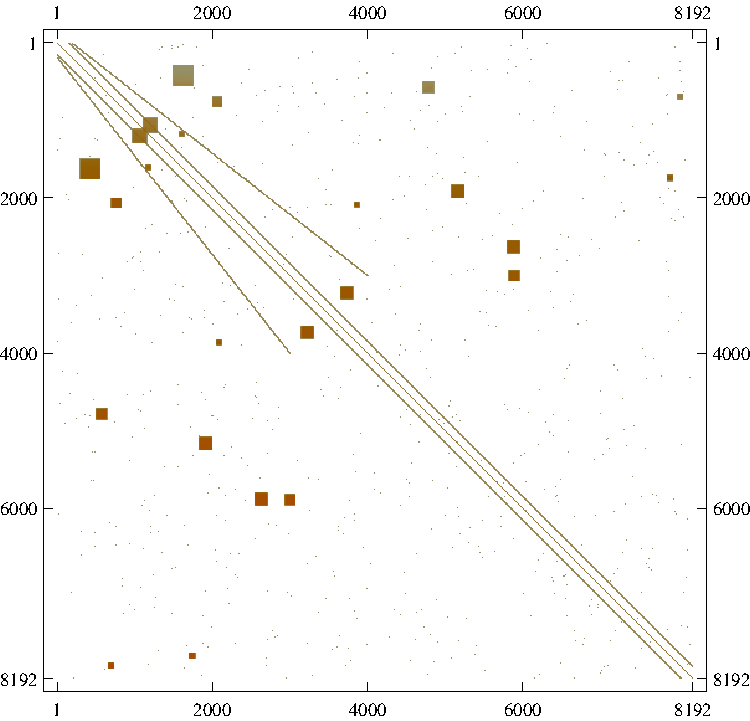
\includegraphics[width=1.0\textwidth]{./images/generated_matrix}
%	\caption{Matice vygenerovaná generátorem}
%	\label{fig:generatedMtx}
%\end{figure}

%\section{Možné optimalizace}
%TODO: popsat moznosti optimalizace - napisu jak by to slo optimalizovat, ale ze jsem to neudelal, protoze mi slo o porovnani mezi % formaty


\section{Měření}

Měření probíhalo na serveru \texttt{star.fit.cvut.cz}. Měřené parametry byly:
\begin{enumerate}
  \item Procentuální zrychlení výpočtu oproti formátu CSR
  \item Počet uzlů ve stromě KAT matice
  \item Velikost datových struktur matic
\end{enumerate}

V grafech značíme matici KAT jako $KAT.n kat block\_size$. Matici BSR jako $bsr block\_size$. 

Pro měření výsledků byly použity následující matice:

\begin{table}[H]
   \begin{tabular}{llllll}
    Skupina    & Název matice & Velikost & Nenulových prvků            & Oblast                  \\
    \hline
    GHS\_indef 	& exdata\_1 \cite{mtxexdata}    &  6001    & 2.269500 $\cdot 10^6$ & optimalizace \\
    Norris     	& heart1 \cite{mtxheart}       & 3557    & 1.385317 $\cdot 10^6$ & 2D/3D          \\
    Gupta     	& gupta3 \cite{mtxgupta}       &  16783    & 9323427 $\cdot 10^6$ & optimalizace         \\
    JGD\_SPG    	& EX6 \cite{mtxex}       & 6545     & 2.95680 $\cdot 10^5$ & kombinatorika \\
    MKS     		& fp \cite{mtxfp}       & 7548     & 8.34222 $\cdot 10^5$ & elektromagnetika         \\
    Belcastro   	& human-gene2 \cite{mtxhuman}        & 14340    & 1.8068388 $\cdot 10^7$ & graf         \\
    \end{tabular}
\end{table}

\subsection{Rychlost výpočtu}

Graf \ref{fig:mmmspeed} ukazuje zrychlení výpočtu na ukázkových matic oproti násobení ve formátu CSR. Graf \ref{fig:mvmspeed} ukazuje stejný případ pro operaci násobení matice vektorem.

\begin{figure}[H]
	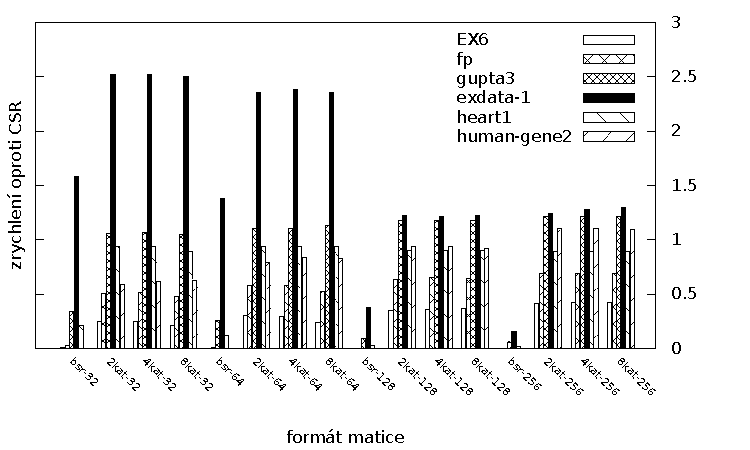
\includegraphics[width=1.0\textwidth]{./images/measure1/mmm-speedup}
	\caption{Zrychlení výpočtu matice $\cdot$ matice oproti formátu CSR}
	\label{fig:mmmspeed}
\end{figure}

\begin{figure}[H]
	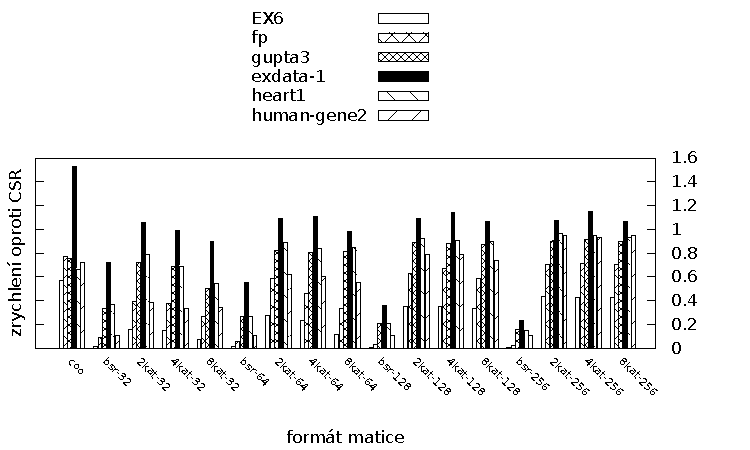
\includegraphics[width=1.0\textwidth]{./images/measure1/mvm-speedup}
	\caption{Zrychlení výpočtu matice $\cdot$ vektor oproti formátu CSR}
	\label{fig:mvmspeed}
\end{figure}

\subsection{Velikost datových struktur}

Graf \ref{fig:mtxsize} ukazuje v bytech přesnou velikost datových struktur matic v porovnání proti uložení matice v hustém formátu. Pro každý prvek bylo potřeba 8B dat, respektive prvky byly uloženy v proměnné typu double.

\begin{figure}[H]
	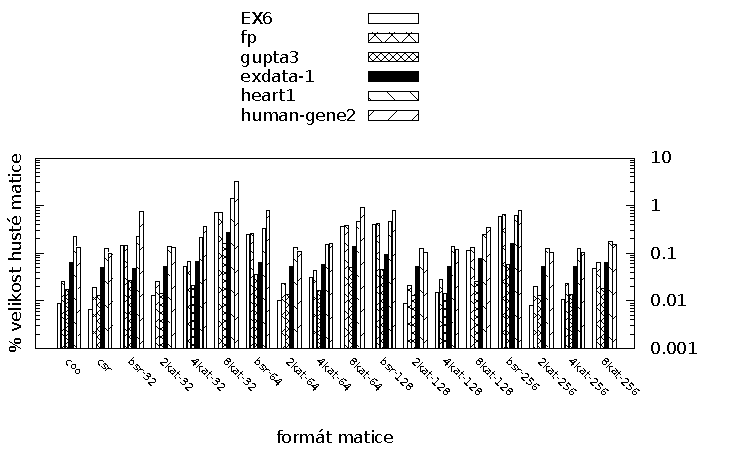
\includegraphics[width=1.0\textwidth]{./images/measure1/ram-up}
	\caption{Velikost datových struktur}
	\label{fig:mtxsize}
\end{figure}

\subsection{Počet uzlů v matici KAT}

Grafy \ref{fig:mtxsizeEX6} \ref{fig:mtxsizeexdata} \ref{fig:mtxsizefp} \ref{fig:mtxsizegupta} \ref{fig:mtxsizeheart} \ref{fig:mtxsizehuman} ukazují počet uzlů ve stromě a jejich druh.

\begin{figure}[htb]
	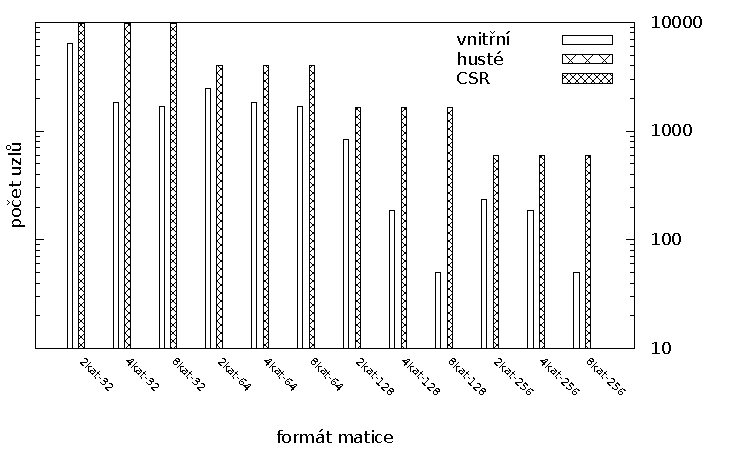
\includegraphics[width=1.0\textwidth]{./images/measure1/kat_nodes_EX6}
	\caption{Počet uzlů v matici KAT pro uložení matice EX6}
	\label{fig:mtxsizeEX6}
\end{figure}

\begin{figure}[htb]
	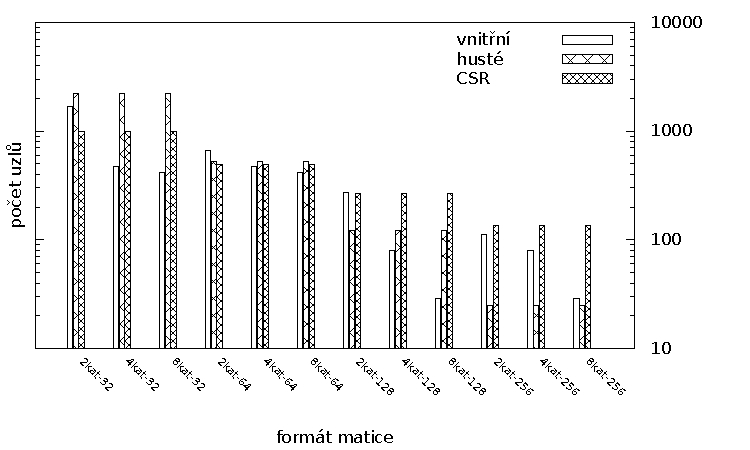
\includegraphics[width=1.0\textwidth]{./images/measure1/kat_nodes_exdata-1}
	\caption{Počet uzlů v matici KAT pro uložení matice exdata-1}
	\label{fig:mtxsizeexdata}
\end{figure}

\begin{figure}[htb]
	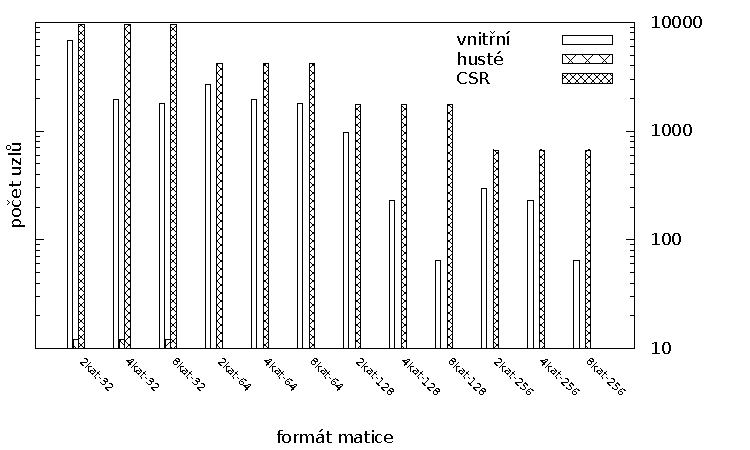
\includegraphics[width=1.0\textwidth]{./images/measure1/kat_nodes_fp}
	\caption{Počet uzlů v matici KAT pro uložení matice fp}
	\label{fig:mtxsizefp}
\end{figure}

\begin{figure}[htb]
	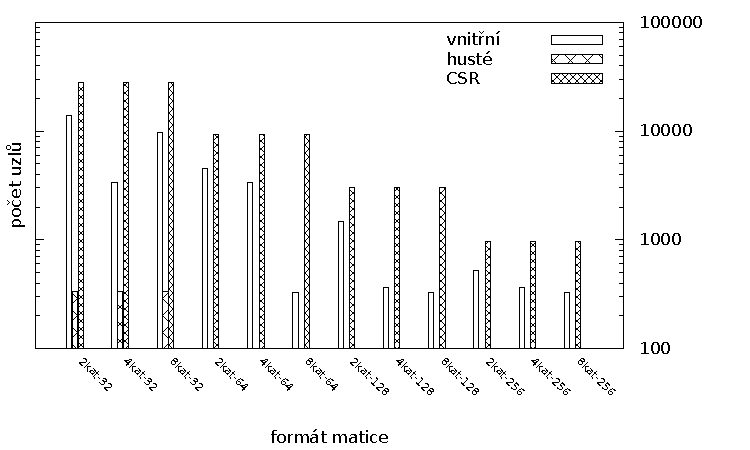
\includegraphics[width=1.0\textwidth]{./images/measure1/kat_nodes_gupta3}
	\caption{Počet uzlů v matici KAT pro uložení matice gupta3}
	\label{fig:mtxsizegupta}
\end{figure}

\begin{figure}[htb]
	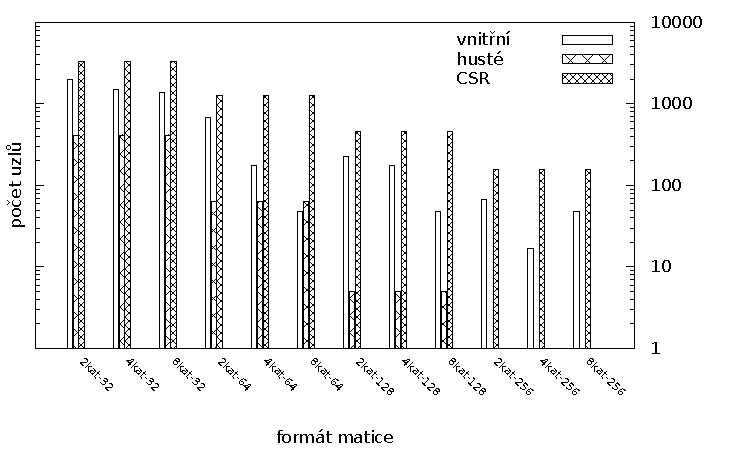
\includegraphics[width=1.0\textwidth]{./images/measure1/kat_nodes_heart1}
	\caption{Počet uzlů v matici KAT pro uložení matice heart1}
	\label{fig:mtxsizeheart}
\end{figure}

\begin{figure}[htb]
	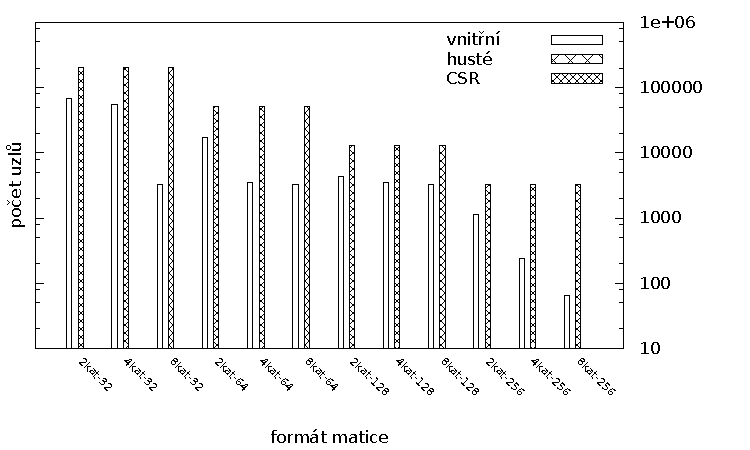
\includegraphics[width=1.0\textwidth]{./images/measure1/kat_nodes_human-gene2}
	\caption{Počet uzlů v matici KAT pro uložení matice human-gene2}
	\label{fig:mtxsizehuman}
\end{figure}


% \begin{sidewaysfigure}
% \end{sidewaysfigure}


\section{Zhodnocení výsledků}

Matice ve formátu BSR dosahovaly velmi špatných výsledků, protože	 její bloky jsou pouze husté. V případě větších bloků s menším počtem nulových prvků tak dochází jak k ukládání těchto nulových prvků zbytečně, tak se tím zpomalí výpočet.

Největším zlepšením byla matice KAT pro matici exdata-1 \cite{mtxexdata}, kde se výpočet zrychlil o více než dvojnásobek. Důvodem bylo efektivní rozdělení matice na husté a řídké části. I paměťová velikost byla srovnatelná s formátem CSR.

U matic, kde není nějaký vzor ve formě bloků, například u matice EX6 \cite{mtxex}, byl formát CSR rychlejší ve všech případech. K za povšimnutí také stojí, že v základním nastavení programu nebyl v matici KAT zvolen pro tuto matici ani jeden hustý list.

Ani jeden hustý list nebyl nebyl zvolen ani pro matici human\_gene2 \cite{mtxhuman}. Vzhledem k její hustotě a velikosti ale pro velké CSR bloky 128 a 256 díky časové a prostorové lokalitě \cite{cachelocal} výsledky lepší než v obyčejném CSR.

Přestože se s větším $k$ u KAT matic výrazně snížil počet vnitřních uzlů, tak se celková datová velikost matice výrazně zvýšila. Důvodem je velikost uzlu, která obsauje $k^2$ ukazatelů na syny. 


%%%%%%%%%%%%%%%%%%%%%%%%%%%%%%%%%%%%%%%%%%%%%%%%%%%%%%%%%%%%%%%%%%%%%%%%%%%%%%
%%%%%%%%%%%%%%%%%%%%%%%%%%%%%%%%%%%%%%%%%%%%%%%%%%%%%%%%%%%%%%%%%%%%%%%%%%%%%%
%%%%%%%%%%%%%%%%%%%%%%%%%%%%%%%%%%%%%%%%%%%%%%%%%%%%%%%%%%%%%%%%%%%%%%%%%%%%%%
%%%%%%%%%%%%%%%%%%%%%%%%%%%%%%%%%%%%%%%%%%%%%%%%%%%%%%%%%%%%%%%%%%%%%%%%%%%%%%
%%%%%%%%%%%%%%%%%%%%%%%%%%%%%%%%%%%%%%%%%%%%%%%%%%%%%%%%%%%%%%%%%%%%%%%%%%%%%%
%%%%%%%%%%%%%%%%%%%%%%%%%%%%%%%%%%%%%%%%%%%%%%%%%%%%%%%%%%%%%%%%%%%%%%%%%% end
%%%%%%%%%%%%%%%%%%%%%%%%%%%%%%%%%%%%%%%%%%%%%%%%%%%%%%%%%%%%%%%%%%%%%%%%%%%%%%
%%%%%%%%%%%%%%%%%%%%%%%%%%%%%%%%%%%%%%%%%%%%%%%%%%%%%%%%%%%%%%%%%%%%%%%%%%%%%%
%%%%%%%%%%%%%%%%%%%%%%%%%%%%%%%%%%%%%%%%%%%%%%%%%%%%%%%%%%%%%%%%%%%%%%%%%%%%%%
%%%%%%%%%%%%%%%%%%%%%%%%%%%%%%%%%%%%%%%%%%%%%%%%%%%%%%%%%%%%%%%%%%%%%%%%%%%%%%
%%%%%%%%%%%%%%%%%%%%%%%%%%%%%%%%%%%%%%%%%%%%%%%%%%%%%%%%%%%%%%%%%%%%%%%%%%%%%%

%\chapter{Cíl práce}

%\chapter{Analýza a návrh}

%\chapter{Realizace}

\begin{conclusion}

Násobení matic je jednoduchá početní úloha, se kterou se setkáme již na střední škole. Pro násobení velkých řídkých matic je pro vyšší výkonnost potřeba  sofistikovanějších algoritmů a rozdělení matic na části.

V této práci jsme popsali základní, ale i pokročilé algoritmy pro násobení matic. Popsali jsme formáty pro uložení řídkých matic COO, CSR, BSR, Quadtree a jeho modifikaci snížením stromu, pojmenovaným KAT. Tyto formáty a algoritmy pro násobení v těchto formátech jsme implementovali a změřili jsme jejich výkonnost na vybraných maticích z praxe.

Měření ukázalo, že násobení matic ve formátu Quadtree a jeho modifikaci do formátu KAT je vhodným formátem, pokud máme dostatek operační paměti a matice buď obsahuje hustší bloky, nebo tolik prvků, že začne využívat cache více než formát CSR.

\section{Další práce}

\subsection{Paralelizace}

Díky paralelizaci by se mohlo u formátu KAT zvýšení rychlosti oproti CSR ještě zvýšit, protože by jednotlivá vlákna řešili jednotlivé bloky a využívali by tak cache efektivněji než CSR. 

\subsection{Strassenův algoritmus}

CSR není vhodný formát pro Strassenův algoritmus. Tento algorimus by ale šel implementovat do formátu Quadtree. Experimentem by mohla být implementace rozbaleného Strassenova algoritmu, tedy místo násobení matic o velikosti $n = 2$ by se násobily rovnou matice o velikosti například $n = 4$. Změněním pořadí operací by mohlo dojít k zefektivnění tohoto algoritmu. 

\subsection{Řídké uzly}
	
V naší implementaci byly uzly matice KAT implementovány jako husté matice ukazatelů na syny. Pro velká $k$ by bylo vhodnější, kdyby i uzly tohoto stromu byly řídké matice.	
	
\end{conclusion}

\bibliographystyle{csn690}
\bibliography{mybibliographyfile}

\appendix

\chapter{Seznam použitých zkratek}
% \printglossaries
\begin{description}
	\item[COO] Coordinate
	\item[BSR] Block sparse row
	\item[CSC] Column sparse column
	\item[CSR] Column sparse row
	\item[KAT] k-ary tree
\end{description}

\nopagebreak[4]
\nopagebreak[4]

% !nesro
\listoffigures

\nopagebreak[4]
\nopagebreak[4]

\listofalgorithms*
% !!nesro

\nopagebreak[4]
\nopagebreak[4]

% % % % % % % % % % % % % % % % % % % % % % % % % % % % 
% % Tuto kapitolu z výsledné práce ODSTRAŇTE.
% % % % % % % % % % % % % % % % % % % % % % % % % % % % 
% 
% \chapter{Návod k~použití této šablony}
% 
% Tento dokument slouží jako základ pro napsání závěrečné práce na Fakultě informačních technologií ČVUT v~Praze.
% 
% \section{Výběr základu}
% 
% Vyberte si šablonu podle druhu práce (bakalářská, diplomová), jazyka (čeština, angličtina) a kódování (ASCII, \mbox{UTF-8}, \mbox{ISO-8859-2} neboli latin2 a nebo \mbox{Windows-1250}). 
% 
% V~české variantě naleznete šablony v~souborech pojmenovaných ve formátu práce\_kódování.tex. Typ může být:
% \begin{description}
% 	\item[BP] bakalářská práce,
% 	\item[DP] diplomová (magisterská) práce.
% \end{description}
% Kódování, ve kterém chcete psát, může být:
% \begin{description}
% 	\item[UTF-8] kódování Unicode,
% 	\item[ISO-8859-2] latin2,
% 	\item[Windows-1250] znaková sada 1250 Windows.
% \end{description}
% V~případě nejistoty ohledně kódování doporučujeme následující postup:
% \begin{enumerate}
% 	\item Otevřete šablony pro kódování UTF-8 v~editoru prostého textu, který chcete pro psaní práce použít -- pokud můžete texty s~diakritikou normálně přečíst, použijte tuto šablonu.
% 	\item V~opačném případě postupujte dále podle toho, jaký operační systém používáte:
% 	\begin{itemize}
% 		\item v~případě Windows použijte šablonu pro kódování \mbox{Windows-1250},
% 		\item jinak zkuste použít šablonu pro kódování \mbox{ISO-8859-2}.
% 	\end{itemize}
% \end{enumerate}
% 
% 
% V~anglické variantě jsou šablony pojmenované podle typu práce, možnosti jsou:
% \begin{description}
% 	\item[bachelors] bakalářská práce,
% 	\item[masters] diplomová (magisterská) práce.
% \end{description}
% 
% \section{Použití šablony}
% 
% Šablona je určena pro zpracování systémem \LaTeXe{}. Text je možné psát v~textovém editoru jako prostý text, lze však také využít specializovaný editor pro \LaTeX{}, např. Kile.
% 
% Pro získání tisknutelného výstupu z~takto vytvořeného souboru použijte příkaz \verb|pdflatex|, kterému předáte cestu k~souboru jako parametr. Vhodný editor pro \LaTeX{} toto udělá za Vás. \verb|pdfcslatex| ani \verb|cslatex| \emph{nebudou} s~těmito šablonami fungovat.
% 
% Více informací o~použití systému \LaTeX{} najdete např. v~\cite{wikilatex}.
% 
% \subsection{Typografie}
% 
% Při psaní dodržujte typografické konvence zvoleného jazyka. České \uv{uvozovky} zapisujte použitím příkazu \verb|\uv|, kterému v~parametru předáte text, jenž má být v~uvozovkách. Anglické otevírací uvozovky se v~\LaTeX{}u zadávají jako dva zpětné apostrofy, uzavírací uvozovky jako dva apostrofy. Často chybně uváděný symbol "{} (palce) nemá s~uvozovkami nic společného.
% 
% Dále je třeba zabránit zalomení řádky mezi některými slovy, v~češtině např. za jednopísmennými předložkami a spojkami (vyjma \uv{a}). To docílíte vložením pružné nezalomitelné mezery -- znakem \texttt{\textasciitilde}. V~tomto případě to není třeba dělat ručně, lze použít program \verb|vlna|.
% 
% Více o~typografii viz \cite{kobltypo}.
% 
% \subsection{Obrázky}
% 
% Pro umožnění vkládání obrázků je vhodné použít balíček \verb|graphicx|, samotné vložení se provede příkazem \verb|\includegraphics|. Takto je možné vkládat obrázky ve formátu PDF, PNG a JPEG jestliže používáte pdf\LaTeX{} nebo ve formátu EPS jestliže používáte \LaTeX{}. Doporučujeme preferovat vektorové obrázky před rastrovými (vyjma fotografií).
% 
% \subsubsection{Získání vhodného formátu}
% 
% Pro získání vektorových formátů PDF nebo EPS z~jiných lze použít některý z~vektorových grafických editorů. Pro převod rastrového obrázku na vektorový lze použít rasterizaci, kterou mnohé editory zvládají (např. Inkscape). Pro konverze lze použít též nástroje pro dávkové zpracování běžně dodávané s~\LaTeX{}em, např. \verb|epstopdf|.
% 
% \subsubsection{Plovoucí prostředí}
% 
% Příkazem \verb|\includegraphics| lze obrázky vkládat přímo, doporučujeme však použít plovoucí prostředí, konkrétně \verb|figure|. Například obrázek \ref{fig:float} byl vložen tímto způsobem. Vůbec přitom nevadí, když je obrázek umístěn jinde, než bylo původně zamýšleno -- je tomu tak hlavně kvůli dodržení typografických konvencí. Namísto vynucování konkrétní pozice obrázku doporučujeme používat odkazování z~textu (dvojice příkazů \verb|\label| a \verb|\ref|).
% 
% \begin{figure}\centering
% 	
\includegraphics[width=0.5\textwidth, angle=30]{cvut-logo-bw}
% 	\caption[Příklad obrázku]{Ukázkový obrázek v~plovoucím prostředí}\label{fig:float}
% \end{figure}
% 
% \subsubsection{Verze obrázků}
% 
% % Gnuplot BW i barevně
% Může se hodit mít více verzí stejného obrázku, např. pro barevný či černobílý tisk a nebo pro prezentaci. S~pomocí některých nástrojů na generování grafiky je to snadné.
% 
% Máte-li například graf vytvořený v programu Gnuplot, můžete jeho černobílou variantu (viz obr. \ref{fig:gnuplot-bw}) vytvořit parametrem \verb|monochrome dashed| příkazu \verb|set term|. Barevnou variantu (viz obr. \ref{fig:gnuplot-col}) vhodnou na prezentace lze vytvořit parametrem \verb|colour solid|.
% 
% \begin{figure}\centering
% 	\includegraphics{gnuplot-bw}
% 	\caption{Černobílá varianta obrázku generovaného programem Gnuplot}\label{fig:gnuplot-bw}
% \end{figure}
% 
% \begin{figure}\centering
% 	\includegraphics{gnuplot-col}
% 	\caption{Barevná varianta obrázku generovaného programem Gnuplot}\label{fig:gnuplot-col}
% \end{figure}
% 
% 
% \subsection{Tabulky}
% 
% Tabulky lze zadávat různě, např. v~prostředí \verb|tabular|, avšak pro jejich vkládání platí to samé, co pro obrázky -- použijte plovoucí prostředí, v~tomto případě \verb|table|. Například tabulka \ref{tab:matematika} byla vložena tímto způsobem.
% 
% \begin{table}\centering
% 	\caption[Příklad tabulky]{Zadávání matematiky}\label{tab:matematika}
% 	\begin{tabular}{|l|l|c|c|}\hline
% 		Typ		& Prostředí		& \LaTeX{}ovská zkratka	& \TeX{}ovská zkratka	\tabularnewline \hline \hline
% 		Text		& \verb|math|		& \verb|\(...\)|	& \verb|$...$|		\tabularnewline \hline
% 		Displayed	& \verb|displaymath|	& \verb|\[...\]|	& \verb|$$...$$|	\tabularnewline \hline
% 	\end{tabular}
% \end{table}
% 
% % % % % % % % % % % % % % % % % % % % % % % % % % % % 

\chapter{Obsah přiloženého CD}

%upravte podle skutecnosti

\begin{figure}
	\dirtree{%
		.1 readme.txt\DTcomment{stručný popis obsahu CD}.
		.1 exe\DTcomment{adresář se spustitelnou formou implementace}.
		.1 src.
		.2 impl\DTcomment{zdrojové kódy implementace}.
		.2 thesis\DTcomment{zdrojová forma práce ve formátu \LaTeX{}}.
		.1 text\DTcomment{text práce}.
		.2 thesis.pdf\DTcomment{text práce ve formátu PDF}.
		.2 thesis.ps\DTcomment{text práce ve formátu PS}.
	}
\end{figure}

\end{document}
